\chapter{พีชคณิตบูลีน (Boolean Algebra)}
\label{ch:boolean}

พีชคณิตบูลีน (Boolean Algebra) เป็นระบบคณิตศาสตร์ที่ศึกษาเกี่ยวกับค่าทางตรรกศาสตร์ 2 สถานะ ได้แก่ 0 (เท็จ) และ 1 (จริง) รวมถึงการดำเนินการทางตรรกะพื้นฐาน โดยพีชคณิตบูลีนทำหน้าที่เป็นรากฐานสำคัญในการออกแบบวงจรดิจิทัล การสร้างเงื่อนไขควบคุมในโปรแกรมคอมพิวเตอร์ และการสืบค้นข้อมูลในระบบฐานข้อมูล~\parencite{mano2018digital}

พีชคณิตบูลีนมีความเชื่อมโยงโดยตรงกับทฤษฎีเซตและตรรกศาสตร์ประพจน์ โดยค่า 0 สอดคล้องกับเซตว่าง ($\emptyset$) ในทฤษฎีเซตและประพจน์ที่เป็นเท็จ ($\bot$) ในตรรกศาสตร์ ในขณะที่ค่า 1 สอดคล้องกับเอกภพสัมพัทธ์ ($U$) และประพจน์ที่เป็นจริง ($\top$) ดังแสดงการเปรียบเทียบในตารางที่~\ref{tab:boolean-set-logic}

เมื่อกำหนดเอกภพสัมพัทธ์ $U$ และเซตย่อย $A, B \subseteq U$ จะพบว่าการดำเนินการ OR สอดคล้องกับยูเนียน ($A \cup B$), การดำเนินการ AND สอดคล้องกับอินเตอร์เซกชัน ($A \cap B$) และการดำเนินการ NOT สอดคล้องกับคอมพลีเมนต์ ($A^c = U - A$) ความสอดคล้องกันนี้ช่วยให้ผู้เรียนสามารถประยุกต์ใช้แนวคิดและกฎทางคณิตศาสตร์ชุดเดียวกันในการทำความเข้าใจทั้งตรรกศาสตร์ ทฤษฎีเซต และการทำงานของวงจรดิจิทัล

\begin{table}[!htb]
    \centering
    \caption{ความสัมพันธ์ระหว่างพีชคณิตบูลีน ทฤษฎีเซต และตรรกศาสตร์}
    \label{tab:boolean-set-logic}
    \begin{tabular}{|c|c|c|}
        \hline
        พีชคณิตบูลีน & ทฤษฎีเซต & ตรรกศาสตร์ประพจน์ \\
        \hline
        0 (เท็จ) & $\emptyset$ (เซตว่าง) & $\bot$ (เท็จ) \\
        \hline
        1 (จริง) & $U$ (เอกภพสัมพัทธ์) & $\top$ (จริง) \\
        \hline
        การดำเนินการ OR ($+$) & ยูเนียน ($\cup$) & การดำเนินการ OR ($\lor$) \\
        \hline
        การดำเนินการ AND ($\cdot$) & อินเตอร์เซกชัน ($\cap$) & การดำเนินการ AND ($\land$) \\
        \hline
        การดำเนินการ NOT ($\overline{x}$) & คอมพลีเมนต์ ($A^c$) & การดำเนินการ NOT ($\neg$) \\
        \hline
    \end{tabular}
\end{table}

\section{นิยามพื้นฐานของพีชคณิตบูลีน}
\label{sec:boolean-definitions}

พีชคณิตบูลีนประกอบด้วยองค์ประกอบหลัก 3 ส่วน ได้แก่ เซตของค่าคงตัวที่ตัวแปรสามารถรับค่าได้ ตัวดำเนินการที่กระทำกับค่าเหล่านั้น และสัจพจน์หรือกฎพื้นฐานที่กำกับการดำเนินการ หัวข้อนี้จะนำเสนอโครงสร้างเชิงพีชคณิตบูลีนอย่างเป็นทางการ พร้อมทั้งอธิบายความหมายของค่าคงตัวทั้งสองค่า เพื่อเป็นพื้นฐานในการศึกษาหัวข้อถัดไปตลอดทั้งบทเรียน~\parencite{mano2018digital}

\subsection{นิยามของพีชคณิตบูลีน}
พีชคณิตบูลีนเป็นโครงสร้างเชิงพีชคณิตที่กำหนดขึ้นเพื่ออธิบายกระบวนการให้เหตุผลเชิงตรรกะและการทำงานของระบบดิจิทัล โดยประกอบด้วยค่าพื้นฐานเพียง 2 ค่าและการดำเนินการตรรกะ พร้อมทั้งสัจพจน์ (Axioms) ที่ควบคุมการดำเนินการเหล่านั้น ข้อแตกต่างสำคัญระหว่างพีชคณิตบูลีนกับพีชคณิตของจำนวนจริง คือ ตัวแปรในพีชคณิตบูลีนสามารถมีค่าได้เพียงสองสถานะเท่านั้น และไม่มีการดำเนินการผกผัน เช่น การลบหรือการหาร ส่งผลให้กฎทางพีชคณิตบางข้อที่ไม่เป็นจริงในระบบจำนวนจริง สามารถเป็นจริงได้ในพีชคณิตบูลีน เช่น กฎการบวกซ้ำ $a + a = a$~\parencite{mano2018digital}

\begin{definition}[พีชคณิตบูลีน]
\index{พีชคณิตบูลีน!นิยาม}
พีชคณิตบูลีน คือ โครงสร้างเชิงพีชคณิต $(B, +, \cdot, ', 0, 1)$ โดยที่ $B$ เป็นเซตที่มีสองสมาชิกคือ $\{0, 1\}$ พร้อมการดำเนินการทวิภาค $+$ และ $\cdot$ และการดำเนินการเอกภาค $'$ โดยสอดคล้องกับสัจพจน์ต่อไปนี้

\begin{enumerate}
    \item กฎการปิด (Closure Laws) สำหรับทุก $a, b \in B$ ได้ว่า
    \begin{enumerate}
        \item $a + b \in B$
        \item $a \cdot b \in B$
    \end{enumerate}
    \item กฎการมีเอกลักษณ์ (Identity Elements)
    \begin{enumerate}
        \item $a + 0 = a$ ($0$ เป็นเอกลักษณ์ของ OR)
        \item $a \cdot 1 = a$ ($1$ เป็นเอกลักษณ์ของ AND)
    \end{enumerate}
    \item กฎการสลับที่ (Commutative Laws)
    \begin{enumerate}
        \item $a + b = b + a$
        \item $a \cdot b = b \cdot a$
    \end{enumerate}
    \item กฎการเปลี่ยนหมู่ (Associative Laws)
    \begin{enumerate}
        \item $(a + b) + c = a + (b + c)$
        \item $(a \cdot b) \cdot c = a \cdot (b \cdot c)$
    \end{enumerate}
    \item กฎการแจกแจง (Distributive Laws)
    \begin{enumerate}
        \item $a \cdot (b + c) = (a \cdot b) + (a \cdot c)$
        \item $a + (b \cdot c) = (a + b) \cdot (a + c)$
    \end{enumerate}
    \item กฎคอมพลีเมนต์ (Complement Laws)
    \begin{enumerate}
        \item $a + a' = 1$
        \item $a \cdot a' = 0$
    \end{enumerate}
\end{enumerate}
\end{definition}

\subsection{ค่าคงตัวบูลีน}
รากฐานของพีชคณิตบูลีนประกอบด้วยค่าคงตัว 2 ค่าที่ใช้แทนสถานะทางตรรกศาสตร์ ได้แก่ เท็จ (0) และจริง (1) ในทางวิศวกรรมฮาร์ดแวร์และวงจรดิจิทัล ค่าทั้งสองจะแทนระดับแรงดันไฟฟ้า 2 ระดับ คือ แรงดันระดับต่ำ (Low Voltage) และแรงดันระดับสูง (High Voltage) การจำกัดค่าของสัญญาณให้อยู่ใน 2 สถานะนี้ ช่วยให้อุปกรณ์อิเล็กทรอนิกส์ เช่น ทรานซิสเตอร์ สามารถทำงานได้อย่างแม่นยำและทนทานต่อสัญญาณรบกวนได้ดีกว่าการประมวลผลสัญญาณหลายระดับ~\parencite{mano2018digital}

\begin{definition}[ค่าคงตัวบูลีน]
\index{ค่าคงตัวบูลีน!นิยาม}
ในพีชคณิตบูลีน มีค่าคงตัวสองค่า ดังนี้
\begin{enumerate}
    \item 0 แทนค่าความจริงเท็จ หรือแรงดันระดับต่ำ
    \item 1 แทนค่าความจริงจริง หรือแรงดันระดับสูง
\end{enumerate}
\end{definition}

\begin{ex}[ความหมายของ 0 และ 1 ในบริบทต่าง ๆ]
\label{ex:bool-constants-meaning}
จงอธิบายความหมายของ 0 และ 1 ในบริบทตรรกศาสตร์ วงจรดิจิทัล และทฤษฎีเซต
\end{ex}
\begin{solution}
ในวงจรดิจิทัล สัญลักษณ์ $0$ แทนแรงดันระดับต่ำ (Low) และ $1$ แทนแรงดันระดับสูง (High); ในตรรกศาสตร์ประพจน์ $0$ แทนค่าความจริงที่เป็นเท็จ ($\bot$) และ $1$ แทนค่าความจริงที่เป็นจริง ($\top$); ในทฤษฎีเซต $0$ สอดคล้องกับเซตว่าง ($\emptyset$) และ $1$ สอดคล้องกับเอกภพสัมพัทธ์ ($U$) โดยระดับแรงดันไฟฟ้าจริงในวงจรดิจิทัลจะขึ้นอยู่กับมาตรฐานเทคโนโลยีของวงจร เช่น ระบบ TTL ($0\text{ V}$ และ $5\text{ V}$) หรือระบบ CMOS ($0\text{ V}$ และ $3.3\text{ V}$)

$\therefore$ ค่า 0 และ 1 เป็นสัญลักษณ์เดียวกันที่ตีความต่างกันตามบริบท คือค่าความจริง ระดับแรงดัน และเซตว่างกับเอกภพสัมพัทธ์ \solhere
\end{solution}

\section{การดำเนินการทางบูลีน (Boolean Operations)}
\label{sec:boolean-operations}

การดำเนินการทางบูลีนถือเป็นแกนหลักของการคำนวณในพีชคณิตบูลีน แม้ว่าชื่อและตารางค่าความจริงของตัวดำเนินการ OR, AND, NOT และ XOR จะมีความสอดคล้องกับตัวเชื่อมทางตรรกศาสตร์ ($\lor, \land, \neg, \oplus$) ในบทที่ผ่านมา แต่ในพีชคณิตบูลีนจะพิจารณาตัวดำเนินการเหล่านี้ในฐานะการคำนวณทางพีชคณิตบนเซต $\{0, 1\}$ หรือที่เรียกว่า \textbf{พีชคณิตสวิตช์ชิง (Switching Algebra)} โดยกำหนดให้สัญลักษณ์ $+$ สอดคล้องกับการต่อสวิตช์ไฟฟ้าแบบขนาน (Parallel Switches), สัญลักษณ์ $\cdot$ สอดคล้องกับการต่อสวิตช์ไฟฟ้าแบบอนุกรม (Series Switches) และสัญลักษณ์ $'$ สอดคล้องกับตัวกลับสัญญาณหรืออินเวอร์เตอร์ (Inverter) การแทนค่าการทำงานของวงจรด้วยสัญลักษณ์ทางพีชคณิตเช่นนี้ ช่วยให้สามารถใช้กฎและเอกลักษณ์ทางคณิตศาสตร์มาจัดรูปและลดทอนความซับซ้อนของวงจรดิจิทัลได้อย่างมีประสิทธิภาพ~\parencite{mano2018digital}

ตารางค่าความจริง (Truth Table) เป็นเครื่องมือพื้นฐานที่ใช้แสดงผลลัพธ์ของการดำเนินการสำหรับทุกกรณีที่เป็นไปได้ของตัวแปรขาเข้า (Input) โดยหากมีตัวแปรจำนวน $n$ ตัว ตารางค่าความจริงจะมีจำนวนกรณีเท่ากับ $2^n$ แถว เช่น ระบบ 2 ตัวแปรจะมี 4 แถว ($2^2 = 4$) และระบบ 3 ตัวแปรจะมี 8 แถว ($2^3 = 8$) การอ่านและสร้างตารางค่าความจริงได้อย่างถูกต้องถือเป็นทักษะสำคัญในการวิเคราะห์และออกแบบวงจรดิจิทัล

\subsection{การดำเนินการ OR (Disjunction)}
การดำเนินการ OR สอดคล้องกับตัวเชื่อม ``หรือ'' ในตรรกศาสตร์ โดยให้ผลลัพธ์เป็น 1 เมื่อมีตัวแปรตัวใดตัวหนึ่งหรือทั้งสองตัวมีค่าเป็น 1 และจะให้ผลลัพธ์เป็น 0 เมื่อตัวแปรทุกตัวมีค่าเป็น 0 เท่านั้น ในทางวงจรดิจิทัล การดำเนินการ OR เทียบเท่ากับการต่อสวิตช์ไฟฟ้าแบบขนาน ซึ่งกระแสไฟฟ้าจะสามารถไหลผ่านวงจรได้เมื่อมีสวิตช์อย่างน้อยหนึ่งตัวปิดวงจร (นำกระแส)~\parencite{mano2018digital}

\begin{definition}[การดำเนินการ OR]
\index{การดำเนินการ OR!นิยาม}
การดำเนินการ OR ของ $a$ และ $b$ เขียนแทนด้วย $a + b$ หรือ $a \lor b$ ให้ผลลัพธ์เป็น 1 ถ้าอย่างน้อยหนึ่งใน $a$ หรือ $b$ เป็น 1 และให้ผลลัพธ์เป็น 0 ก็ต่อเมื่อ $a = b = 0$
\end{definition}

ตารางค่าความจริงของ OR เป็นดังนี้
\begin{center}
\begin{tabular}{|c|c|c|}
\hline
$a$ & $b$ & $a + b$ \\
\hline
0 & 0 & 0 \\
\hline
0 & 1 & 1 \\
\hline
1 & 0 & 1 \\
\hline
1 & 1 & 1 \\
\hline
\end{tabular}
\end{center}

\begin{ex}[การหาค่าของนิพจน์บูลีนที่ใช้ตัวดำเนินการ OR]
\label{ex:eval-or-expression}
จงคำนวณค่าของนิพจน์บูลีน $f(a, b, c) = (a + b) + (a + c)$ เมื่อ $a = 0, b = 1, c = 0$ พร้อมอธิบายสถานะการนำกระแสของวงจรสวิตช์
\end{ex}
\begin{solution}
แทนค่าตัวแปรลงในนิพจน์ตามลำดับ
\begin{align*}
f(0, 1, 0) &= (0 + 1) + (0 + 0) \\
           &= 1 + 0 = 1
\end{align*}
ในเชิงวงจรสวิตช์ไฟฟ้า แม้สวิตช์ $a$ และ $c$ จะเปิดวงจร ($0$) แต่สวิตช์ $b$ ปิดวงจร ($1$) กระแสไฟฟ้าจึงสามารถไหลผ่านเส้นทางขนานเส้นแรกได้สำเร็จ ทำให้ผลลัพธ์โดยรวมเป็น $1$ (แรงดันระดับสูง)

$\therefore f(0,1,0) = 1$ \solhere
\end{solution}

\begin{prop}[สมบัติของ OR]
สำหรับทุก $a, b, c \in \{0, 1\}$ โดยที่ $a, b, c$ แทนค่าบูลีนใด ๆ ดังนี้

\begin{enumerate}
    \item $a + a = a$ \hfill กฎการนิจพล (Idempotent Law)
    \item $a + 0 = a$ \hfill กฎเอกลักษณ์ (Identity Law)
    \item $a + 1 = 1$ \hfill กฎการครอบงำ (Domination Law)
    \item $a + a' = 1$ \hfill กฎคอมพลีเมนต์ (Complement Law)
    \item $a + b = b + a$ \hfill กฎการสลับที่ (Commutative Law)
    \item $(a + b) + c = a + (b + c)$ \hfill กฎการเปลี่ยนหมู่ (Associative Law)
\end{enumerate}
\end{prop}

\subsection{การดำเนินการ AND (Conjunction)}
การดำเนินการ AND สอดคล้องกับตัวเชื่อม ``และ'' ในตรรกศาสตร์ โดยให้ผลลัพธ์เป็น 1 ก็ต่อเมื่อตัวแปรทุกตัวมีค่าเป็น 1 พร้อมกันทั้งหมด และจะให้ผลลัพธ์เป็น 0 หากมีตัวแปรตัวใดตัวหนึ่งเป็น 0 ในทางวงจรดิจิทัล การดำเนินการ AND เทียบเท่ากับการต่อสวิตช์ไฟฟ้าแบบอนุกรม ซึ่งกระแสไฟฟ้าจะสามารถไหลผ่านได้ก็ต่อเมื่อสวิตช์ทุกตัวในแถวปิดวงจรพร้อมกันทั้งหมด~\parencite{roth2021logic}

\begin{definition}[การดำเนินการ AND]
\index{การดำเนินการ AND!นิยาม}
การดำเนินการ AND ของ $a$ และ $b$ เขียนแทนด้วย $a \cdot b$ หรือ $ab$ หรือ $a \land b$ ให้ผลลัพธ์เป็น 1 ก็ต่อเมื่อ $a = b = 1$ และให้ผลลัพธ์เป็น 0 ถ้าอย่างน้อยหนึ่งใน $a$ หรือ $b$ เป็น 0
\end{definition}

ตารางค่าความจริงของ AND เป็นดังนี้
\begin{center}
\begin{tabular}{|c|c|c|}
\hline
$a$ & $b$ & $a \cdot b$ \\
\hline
0 & 0 & 0 \\
\hline
0 & 1 & 0 \\
\hline
1 & 0 & 0 \\
\hline
1 & 1 & 1 \\
\hline
\end{tabular}
\end{center}

\begin{ex}[การหาค่าของนิพจน์บูลีนที่ใช้ตัวดำเนินการ AND]
\label{ex:eval-and-expression}
จงคำนวณค่าของนิพจน์บูลีน $g(a, b, c) = a \cdot b \cdot (b + c)$ เมื่อ $a = 1, b = 1, c = 0$
\end{ex}
\begin{solution}
แทนค่าและคำนวณตามลำดับการดำเนินการ
\begin{align*}
g(1, 1, 0) &= 1 \cdot 1 \cdot (1 + 0) \\
           &= 1 \cdot 1 \cdot 1 = 1
\end{align*}
เนื่องจากสวิตช์ $a$ และ $b$ ในแนวอนุกรมปิดวงจรทั้งคู่ และกลุ่มขนาน $(b+c)$ มี $b=1$ นำกระแส กระแสไฟฟ้าจึงไหลผ่านได้ครบวงจร

$\therefore g(1,1,0) = 1$ \solhere
\end{solution}

\begin{prop}[สมบัติของ AND]
สำหรับทุก $a, b, c \in \{0, 1\}$ โดยที่ $a, b, c$ แทนค่าบูลีนใด ๆ ดังนี้

\begin{enumerate}
    \item $a \cdot a = a$ \hfill กฎการนิจพล (Idempotent Law)
    \item $a \cdot 0 = 0$ \hfill กฎการครอบงำ (Domination Law)
    \item $a \cdot 1 = a$ \hfill กฎเอกลักษณ์ (Identity Law)
    \item $a \cdot a' = 0$ \hfill กฎคอมพลีเมนต์ (Complement Law)
    \item $a \cdot b = b \cdot a$ \hfill กฎการสลับที่ (Commutative Law)
    \item $(a \cdot b) \cdot c = a \cdot (b \cdot c)$ \hfill กฎการเปลี่ยนหมู่ (Associative Law)
\end{enumerate}
\end{prop}

\subsection{การดำเนินการ NOT (Negation)}
การดำเนินการ NOT ทำหน้าที่กลับค่าสถานะทางตรรกะจากค่าหนึ่งไปเป็นอีกค่าหนึ่ง สอดคล้องกับการปฏิเสธ ``ไม่'' ในตรรกศาสตร์ โดย NOT จัดเป็นการดำเนินการเอกภาค (Unary Operation) เนื่องจากรับตัวแปรเพียงตัวเดียว ในทางวงจรดิจิทัล การดำเนินการนี้สร้างขึ้นด้วยวงจรอินเวอร์เตอร์ (Inverter) ซึ่งผลิตระดับแรงดันไฟฟ้าขาออกในทิศทางตรงข้ามกับแรงดันขาเข้าเสมอ~\parencite{wakerly2018digital}

\begin{definition}[การดำเนินการ NOT]
\index{การดำเนินการ NOT!นิยาม}
การดำเนินการ NOT ของ $a$ เขียนแทนด้วย $a'$ หรือ $\overline{a}$ หรือ $\neg a$ ให้ผลลัพธ์ตรงข้ามกับ $a$ นั่นคือ ถ้า $a = 0$ แล้ว $a' = 1$ และถ้า $a = 1$ แล้ว $a' = 0$
\end{definition}

ตารางค่าความจริงของ NOT เป็นดังนี้
\begin{center}
\begin{tabular}{|c|c|}
\hline
$a$ & $a'$ \\
\hline
0 & 1 \\
\hline
1 & 0 \\
\hline
\end{tabular}
\end{center}

\begin{ex}[การหาค่าของนิพจน์บูลีนที่มีนิเสธ]
\label{ex:eval-not-expression}
จงคำนวณค่าของนิพจน์บูลีน $h(x, y) = (x \cdot y)' + x' \cdot y$ เมื่อ $(x, y) = (1, 0)$ และ $(x, y) = (1, 1)$
\end{ex}
\begin{solution}
\begin{align*}
\text{กรณี } (x,y)=(1,0):\quad h(1, 0) &= (1 \cdot 0)' + 1' \cdot 0 = 0' + 0 \cdot 0 = 1 + 0 = 1\\
\text{กรณี } (x,y)=(1,1):\quad h(1, 1) &= (1 \cdot 1)' + 1' \cdot 1 = 1' + 0 \cdot 1 = 0 + 0 = 0
\end{align*}

$\therefore h(0,0) = 1$, $h(0,1) = 1$, $h(1,0) = 1$ และ $h(1,1) = 0$ ซึ่งตรงกับตารางค่าความจริงของ NAND \solhere
\end{solution}

\begin{prop}[สมบัติของ NOT]
สำหรับทุก $a \in \{0, 1\}$ โดยที่ $a$ แทนค่าบูลีนใด ๆ ดังนี้

\begin{enumerate}
    \item $a + a' = 1$ \hfill กฎคอมพลีเมนต์ ข้อ 1
    \item $a \cdot a' = 0$ \hfill กฎคอมพลีเมนต์ ข้อ 2
    \item $(a')' = a$ \hfill กฎนิเสธสองชั้น (Double Negation)
    \item $0' = 1$ และ $1' = 0$ \hfill กฎคอมพลีเมนต์ของค่าคงตัว
\end{enumerate}
\end{prop}

\begin{rem}
\textbf{ข้อสังเกต:} สัญลักษณ์ $+$ และ $\cdot$ ในพีชคณิตบูลีนมีความหมายแตกต่างจากพีชคณิตของจำนวนจริงทั่วไป จึงควรระมัดระวังความแตกต่างดังต่อไปนี้

\begin{enumerate}
    \item ในพีชคณิตบูลีน $1 + 1 = 1$ (เนื่องจากเป็นการดำเนินการ OR ทางตรรกะ ไม่ใช่การบวกเลขจำนวนจริงที่ได้ $2$)
    \item ในพีชคณิตบูลีน $1 \cdot 1 = 1$ (สอดคล้องกับการดำเนินการ AND)
    \item ในพีชคณิตบูลีน $1 + 0 = 1$ (สอดคล้องกับการดำเนินการ OR)
\end{enumerate}
\end{rem}

\subsection{การดำเนินการ XOR (Exclusive OR)}

การดำเนินการ XOR (Exclusive OR) มีบทบาทสำคัญในการออกแบบวงจรคำนวณเลขคณิต วงจรตรวจจับข้อผิดพลาด (Parity Bit Checking) และขั้นตอนวิธีการเข้ารหัสลับ (Cryptography) โดย XOR จะให้ผลลัพธ์เป็น 1 ก็ต่อเมื่อตัวแปรขาเข้าทั้งสองตัวมีสถานะที่แตกต่างกัน (ตัวหนึ่งเป็น 0 และอีกตัวหนึ่งเป็น 1) และจะให้ผลลัพธ์เป็น 0 เมื่อตัวแปรทั้งสองตัวมีสถานะเหมือนกัน~\parencite{kolman2008discrete}

\begin{definition}[การดำเนินการ XOR]
\index{การดำเนินการ XOR!นิยาม}
การดำเนินการ XOR ของ $a$ และ $b$ เขียนแทนด้วย $a \oplus b$ ให้ผลลัพธ์เป็น 1 ก็ต่อเมื่อ $a$ และ $b$ มีค่าต่างกัน และให้ผลลัพธ์เป็น 0 เมื่อ $a$ และ $b$ มีค่าเท่ากัน นั่นคือ
\[ a \oplus b = a'b + ab' = (a \land \neg b) \lor (\neg a \land b) \]
\end{definition}
\begin{center}
\begin{tabular}{|c|c|c|}
\hline
$a$ & $b$ & $a \oplus b$ \\
\hline
0 & 0 & 0 \\
\hline
0 & 1 & 1 \\
\hline
1 & 0 & 1 \\
\hline
1 & 1 & 0 \\
\hline
\end{tabular}
\end{center}

\begin{prop}[สมบัติของ XOR]
สำหรับทุก $a, b, c \in \{0, 1\}$ โดยที่ $a, b, c$ แทนค่าบูลีนใด ๆ ดังนี้

\begin{enumerate}
    \item $a \oplus 0 = a$ \hfill กฎเอกลักษณ์ (Identity)
    \item $a \oplus 1 = a'$ \hfill กฎคอมพลีเมนต์ (Complement)
    \item $a \oplus a = 0$ \hfill กฎการทำซ้ำเป็นศูนย์ (Self-Inverse)
    \item $a \oplus a' = 1$ \hfill กฎการผกผัน (Inverse)
    \item $a \oplus b = b \oplus a$ \hfill กฎการสลับที่ (Commutative)
    \item $(a \oplus b) \oplus c = a \oplus (b \oplus c)$ \hfill กฎการเปลี่ยนหมู่ (Associative)
    \item $a \cdot (b \oplus c) = (a \cdot b) \oplus (a \cdot c)$ \hfill กฎการแจกแจงของ AND บน XOR
    \item $(a \oplus b)' = a \oplus b' = a' \oplus b = a \oplus b \oplus 1$ \hfill รูปสมมูลของ XNOR
\end{enumerate}
\end{prop}

\begin{ex}[การหาค่าของ XOR ที่ต่อกันหลายชั้น]
\label{ex:eval-xor-chain}
จงคำนวณ $1 \oplus 0 \oplus 1$ โดยใช้สมบัติการเปลี่ยนหมู่
\end{ex}
\begin{solution}
\begin{align*}
1 \oplus 0 \oplus 1 &= (1 \oplus 0) \oplus 1 \\
                   &= 1 \oplus 1 \quad \text{(จาก } 1 \oplus 0 = 1 \text{)} \\
                   &= 0 \quad \text{(จาก } a \oplus a = 0 \text{)}
\end{align*}

$\therefore 1 \oplus 0 \oplus 1 = 0$ \solhere
\end{solution}

\begin{ex}[การพิสูจน์รูปสมมูลของ XOR ด้วยตารางค่าความจริง]
\label{ex:xor-equivalence}
พิสูจน์ $a \oplus b = a \cdot b' + a' \cdot b$ โดยใช้ ตารางค่าความจริง
\end{ex}
\begin{solution}
สร้างตารางค่าความจริงเปรียบเทียบทั้งสองข้าง
\begin{center}
\begin{tabular}{|c|c|c|c|c|c|c|}
\hline
$a$ & $b$ & $a'$ & $b'$ & $a \cdot b'$ & $a' \cdot b$ & $a \cdot b' + a' \cdot b$ \\
\hline
0 & 0 & 1 & 1 & 0 & 0 & 0 \\
\hline
0 & 1 & 1 & 0 & 0 & 1 & 1 \\
\hline
1 & 0 & 0 & 1 & 1 & 0 & 1 \\
\hline
1 & 1 & 0 & 0 & 0 & 0 & 0 \\
\hline
\end{tabular}
\end{center}
คอลัมน์ $a \cdot b' + a' \cdot b$ ตรงกับ $a \oplus b$ ทุกแถว $\therefore a \oplus b = a \cdot b' + a' \cdot b$ \solhere
\end{solution}

\section{กฎของพีชคณิตบูลีน (Boolean Identities)}
\label{sec:boolean-identities}

กฎและเอกลักษณ์ของพีชคณิตบูลีน (Boolean Identities) เป็นความสัมพันธ์ทางคณิตศาสตร์ที่เป็นจริงสำหรับทุกสถานะของตัวแปรบูลีน โดยสามารถพิสูจน์ความถูกต้องได้ทั้งจากการแจกแจงทุกกรณีผ่านตารางค่าความจริง (Truth Table) หรือการใช้อนุมานตามสัจพจน์และกฎที่ได้พิสูจน์ไว้แล้ว กฎเหล่านี้มีบทบาทสำคัญต่อกระบวนการลดรูปนิพจน์บูลีน (Expression Simplification) ซึ่งเป็นขั้นตอนพื้นฐานในการออกแบบวงจรดิจิทัลให้มีประสิทธิภาพ การลดทอนความซับซ้อนของนิพจน์จะช่วยลดจำนวนลอจิกเกต (Logic Gates) ที่ต้องใช้ในฮาร์ดแวร์ ส่งผลให้วงจรมีขนาดกะทัดรัด ลดการใช้พลังงาน และเพิ่มความเร็วในการประมวลผลสัญญาณ~\parencite{mano2018digital}

กฎพื้นฐานของพีชคณิตบูลีนประกอบด้วยหลายกลุ่มสำคัญ ได้แก่ กฎเอกลักษณ์ (Identity Laws), กฎการครอบงำ (Domination Laws), กฎการนิจพล (Idempotent Laws), กฎคอมพลีเมนต์ (Complement Laws), กฎการสลับที่ (Commutative Laws), กฎการเปลี่ยนหมู่ (Associative Laws), กฎการแจกแจง (Distributive Laws) และกฎการดูดกลืน (Absorption Laws) หัวข้อนี้จะนำเสนอกระบวนการพิสูจน์และตัวอย่างการนำไปใช้งานอย่างเป็นระบบ

เมื่อพิจารณากฎทางพีชคณิตบูลีน จะพบว่ากฎต่าง ๆ มักปรากฏเป็นคู่สมมาตรเสมอ เช่น $x + 0 = x$ ปรากฏควบคู่กับ $x \cdot 1 = x$ และ $x + 1 = 1$ ปรากฏควบคู่กับ $x \cdot 0 = 0$ ลักษณะดังกล่าวเป็นผลมาจากสมบัติเชิงโครงสร้างของสัจพจน์พีชคณิตบูลีน ที่มีความสมมาตรอย่างสมบูรณ์ระหว่างตัวดำเนินการ $+$ และ $\cdot$ ซึ่งนำไปสู่หลักการสำคัญที่เรียกว่า \textbf{หลักการทวิภาค (Duality Principle)}

\begin{principle}[หลักการทวิภาค (Duality Principle)]
\label{prin:duality}
\index{หลักการทวิภาค}
\textbf{คู่ทวิภาค} (dual) ของสมการบูลีนหนึ่ง ๆ คือสมการที่ได้จากการสลับสองอย่างพร้อมกันทั่วทั้งสมการ ดังนี้

\begin{enumerate}
    \item สลับตัวดำเนินการ $+$ กับ $\cdot$
    \item สลับค่าคงตัว $0$ กับ $1$
\end{enumerate}

โดย \textbf{คงตัวแปรและคงคอมพลีเมนต์ไว้ตามเดิม} หลักการทวิภาคระบุว่า

\begin{center}
ถ้าสมการบูลีนใดเป็นจริงสำหรับทุกค่าของตัวแปร คู่ทวิภาคของสมการนั้นก็เป็นจริงด้วยเสมอ
\end{center}

เหตุผลคือสัจพจน์ทุกข้อของพีชคณิตบูลีนมีคู่ทวิภาคของตนเองอยู่ในชุดสัจพจน์แล้ว ดังนั้นการพิสูจน์ใด ๆ ที่อ้างสัจพจน์เป็นลำดับขั้น ย่อมแปลงเป็นการพิสูจน์คู่ทวิภาคได้โดยแทนสัจพจน์แต่ละข้อด้วยคู่ทวิภาคของมันตามลำดับเดิม

ประโยชน์ในทางปฏิบัติของหลักการนี้คือ \textbf{เมื่อพิสูจน์สมการหนึ่งข้อเป็นจริงแล้ว จะได้ความถูกต้องของคู่ทวิภาคโดยอัตโนมัติ} ทำให้กฎทางพีชคณิตบูลีนถูกจัดกลุ่มเป็นคู่ขนานกันเสมอ
\end{principle}

\begin{ex}[การหาคู่ทวิภาคของสมการบูลีน]
\label{ex:duality}
จงหาคู่ทวิภาคของสมการต่อไปนี้ $x + x'y = x + y$
\end{ex}
\begin{solution}
สลับ $+$ เป็น $\cdot$ และ $\cdot$ เป็น $+$ ทุกตำแหน่ง โดยคงตัวแปรและคอมพลีเมนต์ไว้ ในสมการนี้ไม่มีค่าคงตัว $0$ หรือ $1$ จึงไม่ต้องสลับค่าคงตัว ได้

\begin{align*}
x + x'y = x + y \quad \xrightarrow{\ \text{ทวิภาค}\ } \quad x \cdot (x' + y) = x \cdot y
\end{align*}

ตรวจสอบด้วยการไล่ค่า $xy = 00, 01, 10, 11$ ได้ $x(x'+y)$ เป็น $0, 0, 0, 1$ และ $xy$ เป็น $0, 0, 0, 1$ เท่ากันทุกแถว

$\therefore$ คู่ทวิภาคคือ $x(x' + y) = xy$ ซึ่งเป็นจริง สอดคล้องกับหลักการทวิภาค \solhere
\end{solution}

\subsection{กฎการแจกแจง (Distributive Laws)}
กฎการแจกแจงเป็นคุณลักษณะที่แสดงความแตกต่างระหว่างพีชคณิตบูลีนกับพีชคณิตของจำนวนจริงอย่างชัดเจน โดยในระบบจำนวนจริง การคูณสามารถแจกแจงบนการบวกได้เพียงทิศทางเดียว แต่ในพีชคณิตบูลีน การแจกแจงเป็นจริงในทั้งสองทิศทาง กล่าวคือ AND สามารถแจกแจงบน OR ($a \cdot (b + c) = (a \cdot b) + (a \cdot c)$) และ OR สามารถแจกแจงบน AND ($a + (b \cdot c) = (a + b) \cdot (a + c)$) กฎคู่นี้จึงเป็นเครื่องมือสำคัญในการกระจายพจน์และดึงตัวประกอบร่วมเพื่อลดรูปนิพจน์~\parencite{gersting2014structures}

\begin{thrm}[กฎการแจกแจง]
สำหรับทุก $a, b, c \in \{0, 1\}$ โดยที่ $a, b, c$ แทนค่าบูลีนใด ๆ ดังนี้

\begin{enumerate}
    \item $a \cdot (b + c) = (a \cdot b) + (a \cdot c)$ \hfill (AND กระจายเหนือ OR)
    \item $a + (b \cdot c) = (a + b) \cdot (a + c)$ \hfill (OR กระจายเหนือ AND)
\end{enumerate}
\end{thrm}

\begin{proof}
พิสูจน์ข้อ 1 คือ $a \cdot (b + c) = (a \cdot b) + (a \cdot c)$ โดยใช้ตารางค่าความจริง

\begin{center}
\begin{tabular}{|c|c|c|c|c|c|c|c|}
\hline
$a$ & $b$ & $c$ & $b + c$ & $a \cdot (b + c)$ & $a \cdot b$ & $a \cdot c$ & $(a \cdot b) + (a \cdot c)$ \\
\hline
0 & 0 & 0 & 0 & 0 & 0 & 0 & 0 \\
\hline
0 & 0 & 1 & 1 & 0 & 0 & 0 & 0 \\
\hline
0 & 1 & 0 & 1 & 0 & 0 & 0 & 0 \\
\hline
0 & 1 & 1 & 1 & 0 & 0 & 0 & 0 \\
\hline
1 & 0 & 0 & 0 & 0 & 0 & 0 & 0 \\
\hline
1 & 0 & 1 & 1 & 1 & 0 & 1 & 1 \\
\hline
1 & 1 & 0 & 1 & 1 & 1 & 0 & 1 \\
\hline
1 & 1 & 1 & 1 & 1 & 1 & 1 & 1 \\
\hline
\end{tabular}
\end{center}

เนื่องจากคอลัมน์ $a \cdot (b + c)$ และ $(a \cdot b) + (a \cdot c)$ มีค่าเท่ากันทุกแถว ดังนั้น $a \cdot (b + c) = (a \cdot b) + (a \cdot c)$

พิสูจน์ข้อ 2 คือ $a + (b \cdot c) = (a + b) \cdot (a + c)$ โดยใช้ตารางค่าความจริง

\begin{center}
\begin{tabular}{|c|c|c|c|c|c|c|c|}
\hline
$a$ & $b$ & $c$ & $b \cdot c$ & $a + (b \cdot c)$ & $a + b$ & $a + c$ & $(a + b) \cdot (a + c)$ \\
\hline
0 & 0 & 0 & 0 & 0 & 0 & 0 & 0 \\
\hline
0 & 0 & 1 & 0 & 0 & 0 & 1 & 0 \\
\hline
0 & 1 & 0 & 0 & 0 & 1 & 0 & 0 \\
\hline
0 & 1 & 1 & 1 & 1 & 1 & 1 & 1 \\
\hline
1 & 0 & 0 & 0 & 1 & 1 & 1 & 1 \\
\hline
1 & 0 & 1 & 0 & 1 & 1 & 1 & 1 \\
\hline
1 & 1 & 0 & 0 & 1 & 1 & 1 & 1 \\
\hline
1 & 1 & 1 & 1 & 1 & 1 & 1 & 1 \\
\hline
\end{tabular}
\end{center}

เนื่องจากคอลัมน์ $a + (b \cdot c)$ และ $(a + b) \cdot (a + c)$ มีค่าเท่ากันทุกแถว ดังนั้น $a + (b \cdot c) = (a + b) \cdot (a + c)$
\end{proof}

\begin{ex}[การใช้กฎการแจกแจงลดรูปนิพจน์]
\label{ex:distributive-simplify}
จงใช้กฎการแจกแจง $a + (b \cdot c) = (a + b) \cdot (a + c)$ ในการจัดรูปและลดรูปนิพจน์ $f(x, y, z) = (x + y) \cdot (x + y') \cdot (x + z)$
\end{ex}
\begin{solution}
\begin{align*}
f &= [(x + y)(x + y')](x + z) \\
  &= (x + y y')(x + z) \quad \text{(กฎการแจกแจงย้อนกลับ)} \\
  &= (x + 0)(x + z) \quad \text{(กฎคอมพลีเมนต์ } y y' = 0\text{)} \\
  &= x(x + z) \quad \text{(กฎเอกลักษณ์ } x + 0 = x\text{)} \\
  &= x \quad \text{(กฎการดูดกลืน)}
\end{align*}
$\therefore f = x$ \solhere
\end{solution}

\begin{ex}[การพิสูจน์เอกลักษณ์ด้วยกฎการแจกแจง]
\label{ex:prove-absorption-variant}
จงพิสูจน์เอกลักษณ์ $a + a'b = a + b$ โดยใช้กฎการแจกแจงเชิงพีชคณิตบูลีน
\end{ex}
\begin{solution}
\begin{align*}
a + a'b &= (a + a')(a + b) \quad \text{(กฎการแจกแจง } a + bc = (a+b)(a+c)\text{)} \\
        &= 1 \cdot (a + b) \quad \text{(กฎคอมพลีเมนต์ } a + a' = 1\text{)} \\
        &= a + b \quad \text{(กฎเอกลักษณ์ } 1 \cdot x = x\text{)}
\end{align*}
เอกลักษณ์ $a + a'b = a + b$ นี้เป็นหนึ่งในเอกลักษณ์ที่มีประโยชน์มากในการลดรูปนิพจน์บูลีนและวงจรดิจิทัล

$\therefore a + a'b = a + b$ \solhere
\end{solution}

\subsection{กฎการดูดกลืน (Absorption Laws)}
กฎการดูดกลืน (Absorption Laws) แสดงให้เห็นว่านิพจน์ที่มีตัวแปรเดี่ยวเชื่อมโยงกับพจน์ที่มีตัวแปรนั้นเป็นตัวประกอบร่วม สามารถลดรูปลงเหลือเพียงตัวแปรเดี่ยวดังกล่าวได้ เช่น $a + (a \cdot b) = a$ และ $a \cdot (a + b) = a$ กฎนี้มีบทบาทสำคัญในการกำจัดพจน์ที่ซ้ำซ้อนและลดทอนความซับซ้อนของวงจรดิจิทัล~\parencite{rosen2019discrete}

\begin{law}[กฎการดูดกลืน (Absorption Laws)]
สำหรับทุก $a, b \in \{0, 1\}$ โดยที่ $a$ และ $b$ แทนค่าบูลีนใด ๆ ดังนี้

\begin{enumerate}
    \item $a + (a \cdot b) = a$ \hfill (Absorption Law ข้อ 1)
    \item $a \cdot (a + b) = a$ \hfill (Absorption Law ข้อ 2)
\end{enumerate}
\end{law}

\begin{ex}[การพิสูจน์กฎการดูดกลืนรูปที่หนึ่ง]
\label{ex:absorption-law-1}
พิสูจน์กฎการดูดกลืน $a + (a \cdot b) = a$ โดยใช้พีชคณิตบูลีนและ ตารางค่าความจริง
\end{ex}
\begin{solution}
\textbf{วิธีที่ 1 การพิสูจน์เชิงพีชคณิต}
\begin{align*}
a + (a \cdot b) &= (a \cdot 1) + (a \cdot b) \quad \text{(กฎเอกลักษณ์ } a \cdot 1 = a\text{)} \\
                &= a \cdot (1 + b) \quad \text{(กฎการแจกแจงย้อนกลับ)} \\
                &= a \cdot 1 \quad \text{(กฎครอบงำ } 1 + b = 1\text{)} \\
                &= a \quad \text{(กฎเอกลักษณ์)}
\end{align*}
\textbf{วิธีที่ 2 ตารางค่าความจริง}
\begin{center}
\begin{tabular}{|c|c|c|c|c|}
\hline
$a$ & $b$ & $a \cdot b$ & $a + (a \cdot b)$ & $a$ \\
\hline
0 & 0 & 0 & 0 & 0 \\
\hline
0 & 1 & 0 & 0 & 0 \\
\hline
1 & 0 & 0 & 1 & 1 \\
\hline
1 & 1 & 1 & 1 & 1 \\
\hline
\end{tabular}
\end{center}
คอลัมน์ $a + (a \cdot b)$ ตรงกับ $a$ ทุกแถว $\therefore a + (a \cdot b) = a$ \solhere
\end{solution}

\begin{ex}[การพิสูจน์กฎการดูดกลืนรูปที่สอง]
\label{ex:absorption-law-2}
พิสูจน์กฎการดูดกลืน $a \cdot (a + b) = a$ โดยใช้พีชคณิตบูลีนและ ตารางค่าความจริง
\end{ex}
\begin{solution}
\textbf{วิธีที่ 1 การพิสูจน์เชิงพีชคณิต}
\begin{align*}
a \cdot (a + b) &= (a \cdot a) + (a \cdot b) \quad \text{(กฎการแจกแจง)} \\
                &= a + (a \cdot b) \quad \text{(กฎนิจพล } a \cdot a = a\text{)} \\
                &= a \quad \text{(จากกฎการดูดกลืนข้อ 1)}
\end{align*}
\textbf{วิธีที่ 2 ตารางค่าความจริง}
\begin{center}
\begin{tabular}{|c|c|c|c|c|}
\hline
$a$ & $b$ & $a + b$ & $a \cdot (a + b)$ & $a$ \\
\hline
0 & 0 & 0 & 0 & 0 \\
\hline
0 & 1 & 1 & 0 & 0 \\
\hline
1 & 0 & 1 & 1 & 1 \\
\hline
1 & 1 & 1 & 1 & 1 \\
\hline
\end{tabular}
\end{center}
คอลัมน์ $a \cdot (a + b)$ ตรงกับ $a$ ทุกแถว $\therefore a \cdot (a + b) = a$ \solhere
\end{solution}

\section{กฎเดอมอร์แกน (De Morgan's Laws)}


\label{sec:demorgans-laws}

กฎเดอมอร์แกน (De Morgan's Laws) ตั้งชื่อตาม ออกัสตัส เดอมอร์แกน (Augustus De Morgan, ค.ศ. 1806--1871) นักคณิตศาสตร์ชาวอังกฤษ เป็นหนึ่งในกฎพื้นฐานสำคัญของพีชคณิตบูลีน ทำหน้าที่เป็นเครื่องมือหลักในการหาคอมพลีเมนต์ของนิพจน์บูลีนที่ซับซ้อน โดยมีหลักการสำคัญคือ การหาคอมพลีเมนต์ของผลลัพธ์โดยรวมจะเท่ากับการหาคอมพลีเมนต์ของแต่ละตัวแปรก่อน แล้วสลับตัวดำเนินการระหว่าง $+$ กับ $\cdot$~\parencite{mano2018digital}

\begin{thrm}[กฎเดอมอร์แกนสำหรับพีชคณิตบูลีน]
สำหรับทุก $a, b \in \{0, 1\}$ โดยที่ $a$ และ $b$ แทนค่าบูลีนใด ๆ ดังนี้

\begin{enumerate}
    \item $(a + b)' = a' \cdot b'$ \hfill (คอมพลีเมนต์ของ OR เท่ากับ AND ของคอมพลีเมนต์)
    \item $(a \cdot b)' = a' + b'$ \hfill (คอมพลีเมนต์ของ AND เท่ากับ OR ของคอมพลีเมนต์)
\end{enumerate}
\end{thrm}

\begin{proof}
พิสูจน์โดยใช้ตารางค่าความจริง พิจารณาทุกกรณีของ $a$ และ $b$ ดังนี้

สำหรับข้อ 1: $(a + b)' = a' \cdot b'$

\begin{center}
\begin{tabular}{|c|c|c|c|c|c|c|}
\hline
$a$ & $b$ & $a + b$ & $(a + b)'$ & $a'$ & $b'$ & $a' \cdot b'$ \\
\hline
0 & 0 & 0 & 1 & 1 & 1 & 1 \\
\hline
0 & 1 & 1 & 0 & 1 & 0 & 0 \\
\hline
1 & 0 & 1 & 0 & 0 & 1 & 0 \\
\hline
1 & 1 & 1 & 0 & 0 & 0 & 0 \\
\hline
\end{tabular}
\end{center}

เนื่องจากคอลัมน์ $(a + b)'$ และ $a' \cdot b'$ มีค่าเท่ากันทุกแถว ดังนั้น $(a + b)' = a' \cdot b'$

สำหรับข้อ 2: $(a \cdot b)' = a' + b'$

\begin{center}
\begin{tabular}{|c|c|c|c|c|c|c|}
\hline
$a$ & $b$ & $a \cdot b$ & $(a \cdot b)'$ & $a'$ & $b'$ & $a' + b'$ \\
\hline
0 & 0 & 0 & 1 & 1 & 1 & 1 \\
\hline
0 & 1 & 0 & 1 & 1 & 0 & 1 \\
\hline
1 & 0 & 0 & 1 & 0 & 1 & 1 \\
\hline
1 & 1 & 1 & 0 & 0 & 0 & 0 \\
\hline
\end{tabular}
\end{center}

เนื่องจากคอลัมน์ $(a \cdot b)'$ และ $a' + b'$ มีค่าเท่ากันทุกแถว ดังนั้น $(a \cdot b)' = a' + b'$
\end{proof}

สาระสำคัญของกฎเดอมอร์แกนทั้งสองข้อ คือ การใส่นิเสธให้กับนิพจน์โดยรวมจะเทียบเท่ากับการใส่นิเสธให้แก่ตัวแปรย่อยแต่ละตัวแล้วสลับตัวดำเนินการระหว่าง $+$ กับ $\cdot$ ดังแสดงในรูปที่~\ref{fig:boolean-demorgan-flow} ซึ่งในเชิงวงจรดิจิทัลหมายถึง ลอจิกเกตที่ต่อนิเสธไว้ที่สัญญาณขาออก (เช่น เกต NOR หรือ NAND) จะให้ผลการทำงานเทียบเท่ากับลอจิกเกตอีกชนิดหนึ่งที่ต่อนิเสธไว้ที่สัญญาณขาเข้าทุกช่อง

\begin{figure}[H]
    \centering
    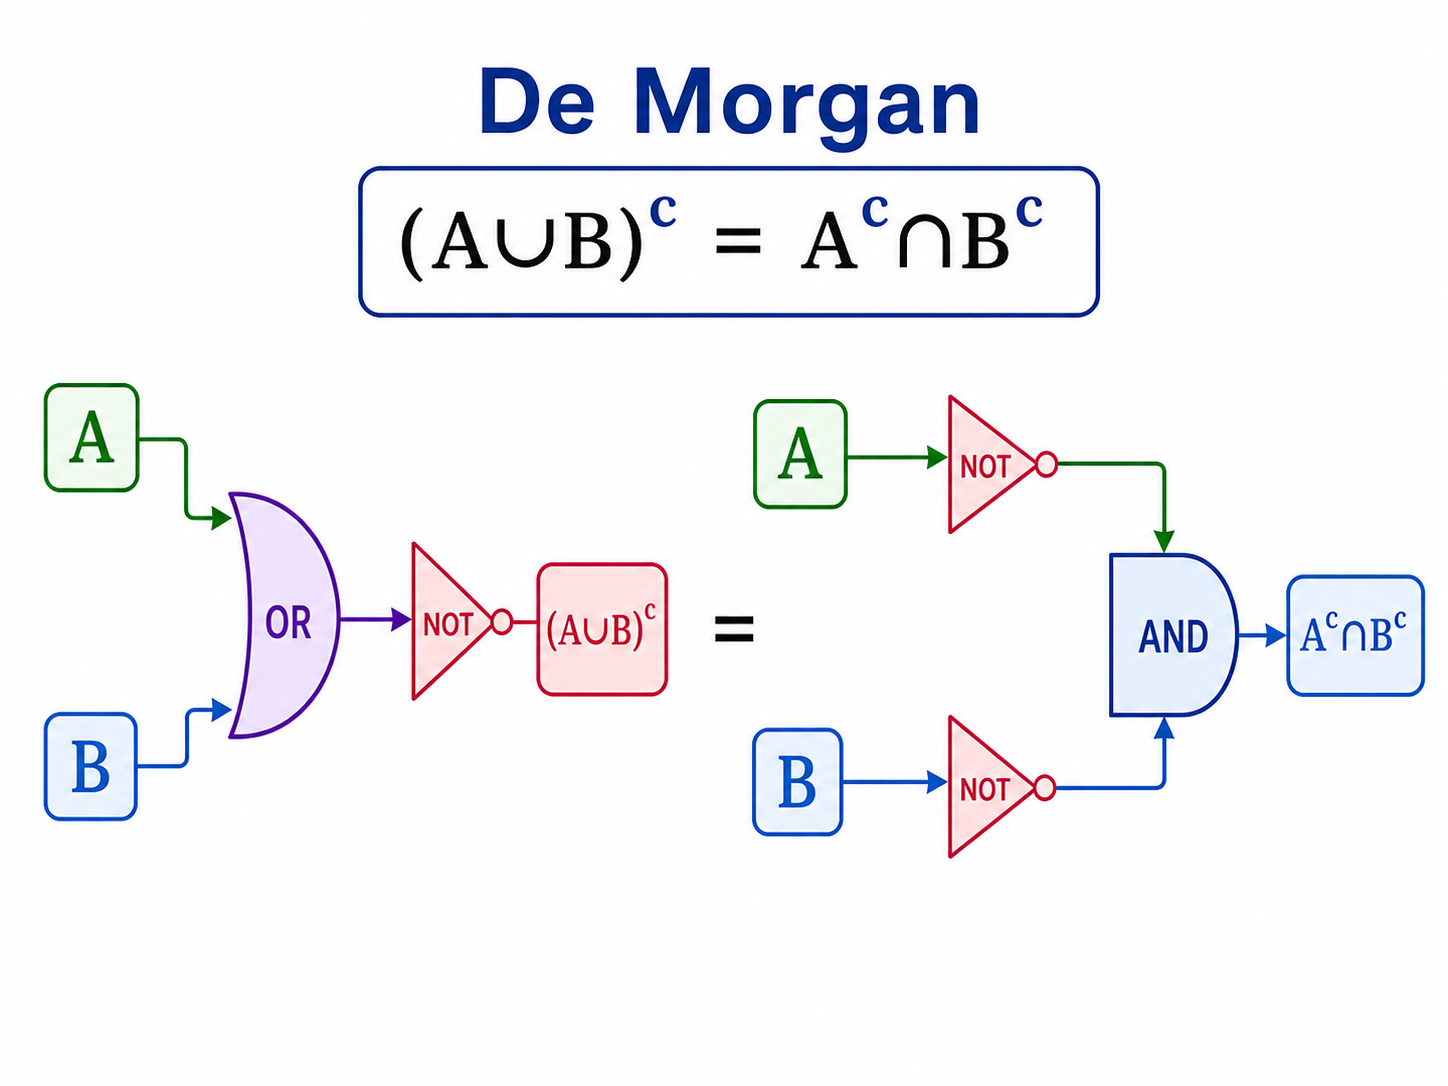
\includegraphics[width=0.82\textwidth]{Figures/png_ready/demorgan-laws-generated.png}
    \caption{กฎเดอมอร์แกน}
    \label{fig:boolean-demorgan-flow}
\end{figure}

\begin{rem}
สังเกตความสอดคล้องกับกฎเดอมอร์แกนในตรรกศาสตร์และทฤษฎีเซต ดังนี้

\begin{enumerate}
    \item $\neg(p \lor q) \equiv \neg p \land \neg q$ สอดคล้องกับ $(a + b)' = a' \cdot b'$
    \item $\neg(p \land q) \equiv \neg p \lor \neg q$ สอดคล้องกับ $(a \cdot b)' = a' + b'$
\end{enumerate}
นี่เป็นตัวอย่างที่แสดงความเชื่อมโยงระหว่างตรรกศาสตร์ ทฤษฎีเซต และพีชคณิตบูลีน
\end{rem}

\section{นิพจน์บูลีนและฟังก์ชันบูลีน (Boolean Expressions and Functions)}
\label{sec:boolean-expressions}
นิพจน์บูลีนและฟังก์ชันบูลีนเป็นเครื่องมือสำคัญในการจำลองและวิเคราะห์ปัญหาทางตรรกศาสตร์ในระบบคอมพิวเตอร์ โดยฟังก์ชันบูลีน (Boolean Function) คือ การจับคู่ (Mapping) จากโดเมนของตัวแปรบูลีน $n$ ตัวแปร $B^n = \{0, 1\}^n$ ไปยังเรนจ์ $\{0, 1\}$ ความสัมพันธ์ของฟังก์ชันสามารถนำเสนอได้ทั้งในรูปของตารางค่าความจริง นิพจน์พีชคณิต และแผนภาพการไหลของสัญญาณ ดังแสดงในรูปที่~\ref{fig:function-mapping}~\parencite{mano2018digital}

รูปที่~\ref{fig:function-mapping} แสดงตัวอย่างการทำงานของฟังก์ชันบูลีน 2 ฟังก์ชันแยกจากกัน โดยแถวบนรับตัวแปรขาเข้า $x$ และ $y$ เพื่อคำนวณ $F = x \cdot y$ (ฟังก์ชัน AND) ส่วนแถวล่างรับตัวแปรขาเข้า $x$ เพื่อคำนวณ $F = \bar{x}$ (ฟังก์ชัน NOT) สัญลักษณ์ $F$ ในแต่ละแถวจึงหมายถึงค่าสัญญาณขาออกของฟังก์ชันนั้น ๆ

\begin{figure}[H]
    \centering
    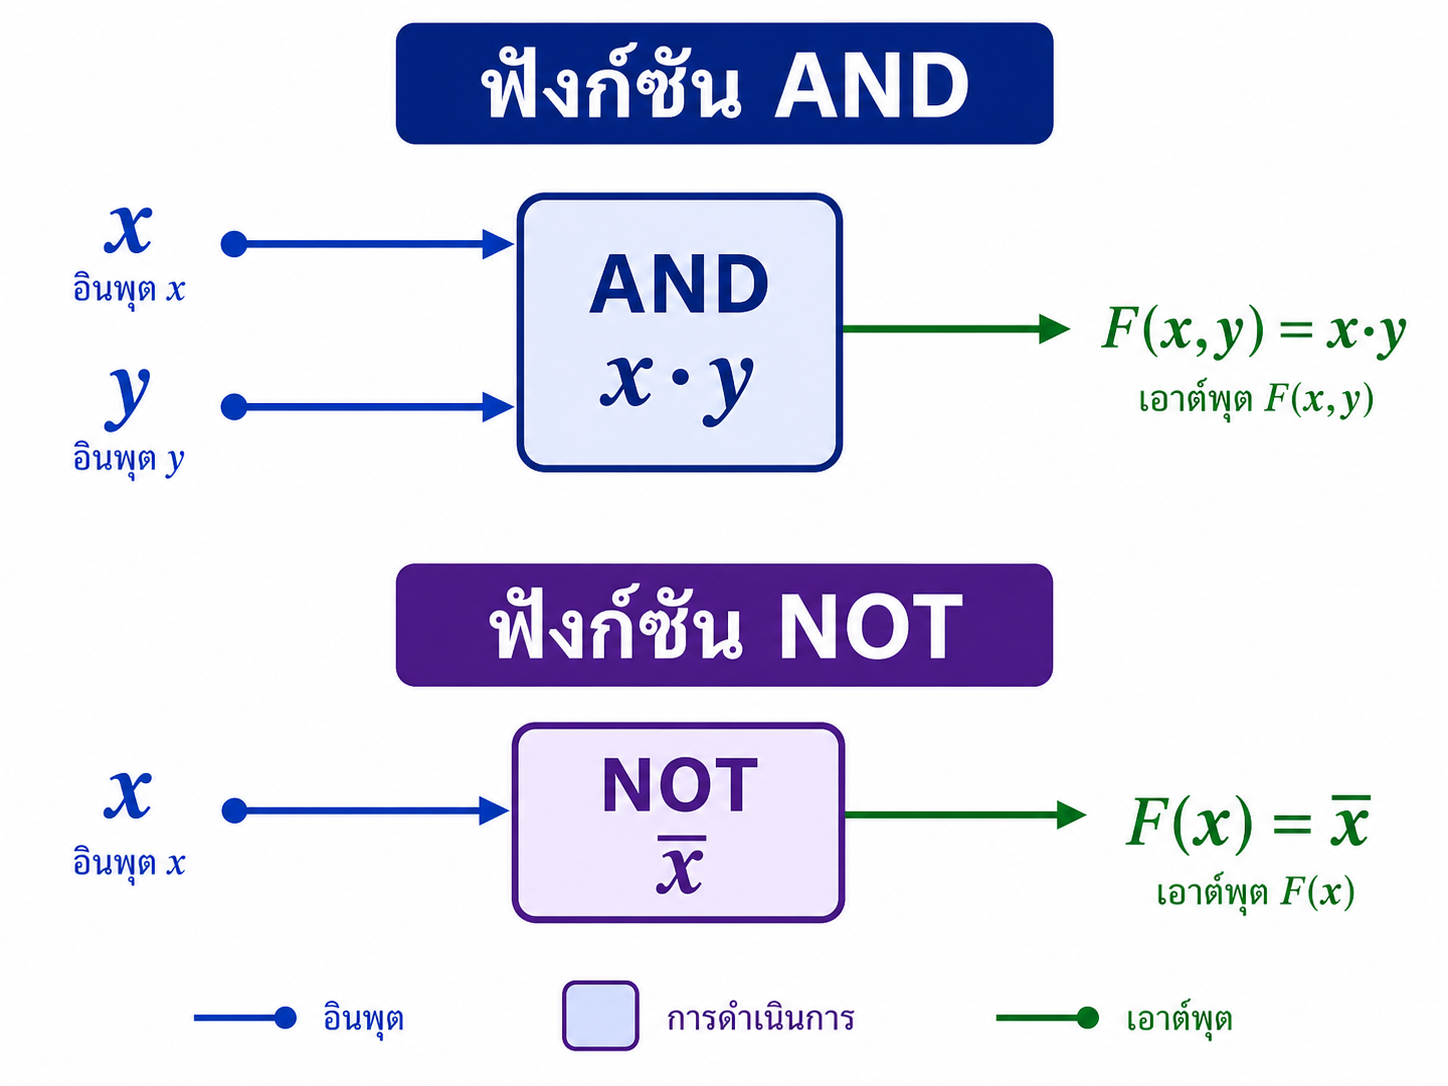
\includegraphics[width=0.78\textwidth]{Figures/png_ready/boolean-function-flow-labeled.png}
    \caption{ตัวอย่างการไหลของอินพุตสำหรับฟังก์ชัน AND และ NOT แยกกัน}
    \label{fig:function-mapping}
\end{figure}

นิพจน์บูลีนประกอบด้วยตัวแปรบูลีน ค่าคงตัว 0 และ 1 พร้อมด้วยตัวดำเนินการ OR, AND และ NOT โดยใช้วงเล็บเพื่อควบคุมลำดับการประมวลผล ฟังก์ชันบูลีนสามารถแสดงผลได้ในหลายรูปแบบ เช่น ตารางค่าความจริง นิพจน์บูลีน และแผนที่คาร์นอ (Karnaugh Map)

ในกระบวนการออกแบบวงจรดิจิทัล ฟังก์ชันบูลีนทำหน้าที่เป็นแบบจำลองเริ่มต้น โดยผู้ออกแบบจะแปลงข้อกำหนดของระบบให้เป็นฟังก์ชันบูลีน จากนั้นจึงดำเนินการลดรูปนิพจน์ให้มีจำนวนพจน์และตัวแปรน้อยที่สุดก่อนนำไปสังเคราะห์เป็นวงจรฮาร์ดแวร์จริง ซึ่งช่วยลดจำนวนอุปกรณ์อิเล็กทรอนิกส์และเกตทางตรรกะ ส่งผลให้วงจรมีขนาดเล็กลง ประหยัดพลังงาน และลดต้นทุนการผลิต

\subsection{นิยามของนิพจน์บูลีน}
นิพจน์บูลีน (Boolean Expression) คือ การนำตัวแปรบูลีน ค่าคงตัว ($0$ และ $1$) และตัวดำเนินการทางตรรกศาสตร์ ($+$, $\cdot$, $'$) มาประกอบเข้าด้วยกันอย่างถูกต้องตามหลักไวยากรณ์ โดยใช้วงเล็บเพื่อกำหนดลำดับการคำนวณ การทำความเข้าใจโครงสร้างและลำดับความสำคัญของตัวดำเนินการในนิพจน์บูลีนเป็นพื้นฐานสำคัญในการวิเคราะห์และสร้างวงจรดิจิทัล~\parencite{mano2018digital}

\begin{definition}[นิพจน์บูลีน]
\index{นิพจน์บูลีน!นิยาม}
นิพจน์บูลีน คือการรวมกันขององค์ประกอบต่อไปนี้
\begin{enumerate}
    \item ตัวแปรบูลีน เช่น $x, y, z$
    \item ค่าคงตัวบูลีน 0 และ 1
    \item การดำเนินการบูลีน ($+$, $\cdot$, $'$)
    \item วงเล็บ $($ และ $)$ เพื่อกำหนดลำดับการดำเนินการ
\end{enumerate}
\end{definition}

\begin{ex}[การจำแนกนิพจน์บูลีนที่ถูกต้องตามกฎการสร้าง]
\label{ex:valid-expressions}
จงตรวจสอบว่านิพจน์ต่อไปนี้เป็นนิพจน์บูลีนที่ถูกต้องตามกฎการสร้างหรือไม่ พร้อมระบุลำดับการดำเนินการ

\begin{enumerate}
    \item $x + y$
    \item $x \cdot y'$
    \item $(x + y) \cdot z$
    \item $x' + y \cdot z$
    \item $(a + b) \cdot (a' + c) + (a \cdot b \cdot c)'$
\end{enumerate}
\end{ex}
\begin{solution}
ทุกนิพจน์สร้างจากตัวแปรบูลีนกับตัวดำเนินการ $+,\ \cdot,\ '$ ตามกฎการสร้างนิพจน์ (ลำดับความสำคัญคือ $'$ ก่อน $\cdot$ ก่อน $+$; วงเล็บกำหนดลำดับได้) $\therefore$ ทั้งห้าเป็นนิพจน์บูลีนที่ถูกต้อง \solhere
\end{solution}

\subsection{ฟังก์ชันบูลีน}
ฟังก์ชันบูลีน (Boolean Function) คือ ฟังก์ชันที่รับค่าตัวแปรขาเข้าเป็นชุดข้อมูลบูลีน และให้ผลลัพธ์ขาออกเป็นค่าบูลีนเพียงค่าเดียว ฟังก์ชันที่มีตัวแปรจำนวน $n$ ตัวจะถูกกำหนดพฤติกรรมได้อย่างสมบูรณ์ด้วยตารางค่าความจริงขนาด $2^n$ แถว ซึ่งแสดงว่าสำหรับตัวแปรจำนวนจำกัด จะมีฟังก์ชันบูลีนที่เป็นไปได้ทั้งหมดจำนวนจำกัดเท่ากับ $2^{2^n}$ ฟังก์ชัน สมบัตินี้ช่วยให้สามารถตรวจสอบความถูกต้องของการทำงานของวงจรได้อย่างครบถ้วนทุกกรณี~\parencite{mano2018digital}

\begin{definition}[ฟังก์ชันบูลีน]
\index{ฟังก์ชันบูลีน!นิยาม}
ฟังก์ชันบูลีน $f(x_1, x_2, \ldots, x_n)$ คือ ฟังก์ชันที่รับค่าบูลีน $n$ ตัวแปรและให้ผลลัพธ์เป็นค่าบูลีน
\end{definition}

ฟังก์ชันบูลีนสามารถแทนด้วยตารางค่าความจริงที่แสดงผลลัพธ์สำหรับทุกชุดค่าอินพุตที่เป็นไปได้

\begin{ex}[การสร้างตารางค่าความจริงของฟังก์ชันสองตัวแปร]
\label{ex:truth-table-2var}
จงสร้างตารางค่าความจริงของ $f(x, y) = x \cdot y + x' \cdot y'$ แล้วระบุว่าฟังก์ชันนี้ตรงกับการดำเนินการมาตรฐานชนิดใด
\end{ex}
\begin{solution}
สร้างตารางค่าความจริงของฟังก์ชัน
\begin{center}
\begin{tabular}{|c|c|c|c|c|c|}
\hline
$x$ & $y$ & $x'$ & $y'$ & $x \cdot y$ & $x \cdot y + x' \cdot y'$ \\
\hline
0 & 0 & 1 & 1 & 0 & 1 \\
\hline
0 & 1 & 1 & 0 & 0 & 0 \\
\hline
1 & 0 & 0 & 1 & 0 & 0 \\
\hline
1 & 1 & 0 & 0 & 1 & 1 \\
\hline
\end{tabular}
\end{center}
$f = 1$ เมื่อ $x = y$ และ $f = 0$ เมื่อ $x \neq y$ $\therefore f$ คือฟังก์ชัน \textbf{XNOR} \solhere
\end{solution}

\begin{ex}[การสร้างตารางค่าความจริงของฟังก์ชันสามตัวแปร]
\label{ex:truth-table-3var}
จงสร้างตารางค่าความจริงของ $f(x, y, z) = (x + y') \cdot z + x \cdot y$ โดยแยกคอลัมน์ของแต่ละพจน์ย่อยเพื่อลดความผิดพลาด
\end{ex}
\begin{solution}
สร้างตารางค่าความจริงของฟังก์ชัน
\begin{center}
\begin{tabular}{|c|c|c|c|c|c|c|c|}
\hline
$x$ & $y$ & $z$ & $y'$ & $x + y'$ & $(x + y') \cdot z$ & $x \cdot y$ & $f$ \\
\hline
0 & 0 & 0 & 1 & 1 & 0 & 0 & 0 \\
\hline
0 & 0 & 1 & 1 & 1 & 1 & 0 & 1 \\
\hline
0 & 1 & 0 & 0 & 0 & 0 & 0 & 0 \\
\hline
0 & 1 & 1 & 0 & 0 & 0 & 0 & 0 \\
\hline
1 & 0 & 0 & 1 & 1 & 0 & 0 & 0 \\
\hline
1 & 0 & 1 & 1 & 1 & 1 & 0 & 1 \\
\hline
1 & 1 & 0 & 0 & 1 & 0 & 1 & 1 \\
\hline
1 & 1 & 1 & 0 & 1 & 1 & 1 & 1 \\
\hline
\end{tabular}
\end{center}

$\therefore$ ตารางค่าความจริงของ $f$ ครบทั้งแปดแถวตามที่แสดง \solhere
\end{solution}

\section{รูปแบบบัญญัติ (Canonical Forms)}
\label{sec:canonical-forms}

รูปแบบบัญญัติ (Canonical Forms) เป็นวิธีมาตรฐานสากลในการแสดงฟังก์ชันบูลีนให้อยู่ในโครงสร้างที่เป็นเอกลักษณ์และเป็นระบบ โดยฟังก์ชันบูลีนใด ๆ สามารถเขียนแสดงในรูปแบบบัญญัติได้ 2 รูปแบบหลัก ได้แก่ รูปแบบผลบวกของผลคูณ (Sum of Products: SOP) และรูปแบบผลคูณของผลบวก (Product of Sums: POS) การเขียนฟังก์ชันในรูปแบบบัญญัตินอกจากจะช่วยให้สามารถเปรียบเทียบความสมมูลของฟังก์ชันได้อย่างชัดเจนแล้ว ยังเป็นพื้นฐานสำคัญในการลดรูปนิพจน์ด้วยแผนที่คาร์นอ (Karnaugh Map)~\parencite{roth2021logic}

\subsection{มินเทอมและแมกซ์เทอม (Minterms and Maxterms)}
การทำความเข้าใจรูปแบบบัญญัติจำเป็นต้องอาศัยแนวคิดพื้นฐานของ \textbf{มินเทอม (Minterm)} และ \textbf{แมกซ์เทอม (Maxterm)} โดยมินเทอมคือพจน์ผลคูณ (AND Term) ที่ประกอบด้วยตัวแปรทุกตัวในฟังก์ชันปรากฏเพียงครั้งเดียว (หากตัวแปรมีค่าเป็น 1 จะแทนด้วยตัวแปรปกติ แต่หากมีค่าเป็น 0 จะแทนด้วยคอมพลีเมนต์) ในทางตรงกันข้าม แมกซ์เทอมคือพจน์ผลบวก (OR Term) ที่ประกอบด้วยตัวแปรทุกตัวปรากฏเพียงครั้งเดียว โดยหากตัวแปรมีค่าเป็น 0 จะแทนด้วยตัวแปรปกติ และหากมีค่าเป็น 1 จะแทนด้วยคอมพลีเมนต์ ความสัมพันธ์ระหว่างมินเทอมและแมกซ์เทอมช่วยให้สามารถแปลงรูปฟังก์ชันระหว่าง SOP และ POS ได้อย่างเป็นระบบ~\parencite{wakerly2018digital}

\begin{definition}[มินเทอม]
\index{มินเทอม!นิยาม}
มินเทอม ของตัวแปร $n$ ตัวคือ AND term ที่มีตัวแปรทุกตัวปรากฏเพียงครั้งเดียวในรูปแบบบัญญัติ (ถ้าตัวแปรเป็น 1 ใช้ตัวแปรเดี่ยว ถ้าตัวแปรเป็น 0 ใช้คอมพลีเมนต์)

สำหรับ 2 ตัวแปร $x, y$ ได้ดังนี้
\begin{enumerate}
    \item $m_0 = x' \cdot y'$ (ทั้ง $x = 0, y = 0$)
    \item $m_1 = x' \cdot y$ (ทั้ง $x = 0, y = 1$)
    \item $m_2 = x \cdot y'$ (ทั้ง $x = 1, y = 0$)
    \item $m_3 = x \cdot y$ (ทั้ง $x = 1, y = 1$)
\end{enumerate}
\end{definition}

\begin{definition}[แมกซ์เทอม]
\index{แมกซ์เทอม!นิยาม}
แมกซ์เทอม ของตัวแปร $n$ ตัวคือ OR term ที่มีตัวแปรทุกตัวปรากฏเพียงครั้งเดียวในรูปแบบบัญญัติ (ถ้าตัวแปรเป็น 0 ใช้ตัวแปรเดี่ยว ถ้าตัวแปรเป็น 1 ใช้คอมพลีเมนต์)

สำหรับ 2 ตัวแปร $x, y$ ได้ดังนี้
\begin{enumerate}
    \item $M_0 = x + y$ (ทั้ง $x = 0, y = 0$)
    \item $M_1 = x + y'$ (ทั้ง $x = 0, y = 1$)
    \item $M_2 = x' + y$ (ทั้ง $x = 1, y = 0$)
    \item $M_3 = x' + y'$ (ทั้ง $x = 1, y = 1$)
\end{enumerate}
\end{definition}

\begin{prop}
ความสัมพันธ์ระหว่าง Minterm และ Maxterm โดยที่ $m_i$ และ $M_i$ แทนมินเทอมและแมกซ์เทอมลำดับที่ $i$ ตามลำดับ
\begin{enumerate}
    \item $m_i = M_i'$
    \item $M_i = m_i'$
    \item $\sum$ (sigma) ใช้แทน sum ของ minterms
    \item $\prod$ (pi) ใช้แทน product ของ maxterms
\end{enumerate}
\end{prop}

\subsection{ผลบวกของผลคูณ (Sum of Products -- SOP)}
รูปแบบผลบวกของผลคูณ (Sum of Products: SOP) เป็นโครงสร้างมาตรฐานที่นิยมใช้ในการออกแบบวงจรดิจิทัล โดยเกิดจากการนำพจน์มินเทอมของแถวที่ฟังก์ชันให้ผลลัพธ์เป็น 1 มารวมกันด้วยตัวดำเนินการ OR (ผลบวกของกลุ่มผลคูณ AND) โครงสร้างในรูปแบบ SOP มีบทบาทสำคัญเนื่องจากสามารถนำไปสังเคราะห์เป็นวงจรดิจิทัลระดับ 2 ชั้น (Two-Level Logic Circuit) ที่ประกอบด้วยเกต AND ในชั้นแรกและเกต OR ในชั้นสุดท้ายได้อย่างสะดวกรวดเร็ว~\parencite{kolman2008discrete}

\begin{definition}[รูปแบบผลบวกของผลคูณ (SOP)]
\index{รูปแบบผลบวกของผลคูณ!นิยาม}
รูปแบบผลบวกของผลคูณ (Sum of Products: SOP) คือ รูปแบบของนิพจน์บูลีนที่เขียนเป็น OR ของ AND terms โดยฟังก์ชันบูลีนใด ๆ สามารถเขียนเป็น SOP ได้โดยใช้ minterm expansion
\end{definition}

\begin{ex}[การเขียนฟังก์ชันในรูปแบบบัญญัติ SOP]
\label{ex:canonical-sop}
เขียนฟังก์ชัน $f(x, y) = x \cdot y + x'$ ในรูปแบบ canonical SOP
\end{ex}
\begin{solution}
สร้างตารางค่าความจริงของฟังก์ชัน
\begin{center}
\begin{tabular}{|c|c|c|c|c|}
\hline
$x$ & $y$ & $x \cdot y$ & $x'$ & $f$ \\
\hline
0 & 0 & 0 & 1 & 1 \\
\hline
0 & 1 & 0 & 1 & 1 \\
\hline
1 & 0 & 0 & 0 & 0 \\
\hline
1 & 1 & 1 & 0 & 1 \\
\hline
\end{tabular}
\end{center}
แถวที่ $f = 1$ ได้แก่ $(0,0), (0,1), (1,1)$ ตรงกับ $m_0 = x'y',\ m_1 = x'y,\ m_3 = xy$
\[
\therefore f(x, y) = x'y' + x'y + xy = \sum(0, 1, 3)
\]
\solhere
\end{solution}

\begin{ex}[การเขียน SOP จากรายการมินเทอม]
\label{ex:sop-from-minterms}
กำหนดให้ตารางค่าความจริงของ $f(x, y, z)$ มีค่า $f = 1$ ที่มินเทอม $m_1, m_3, m_5, m_7$ จงเขียน $f$ ในรูปแบบบัญญัติ SOP
\end{ex}
\begin{solution}
\begin{align*}
m_1 = 001 &\Rightarrow x'y'z & m_3 = 011 &\Rightarrow x'yz\\
m_5 = 101 &\Rightarrow xy'z & m_7 = 111 &\Rightarrow xyz
\end{align*}
$\therefore f(x, y, z) = x'y'z + x'yz + xy'z + xyz = \sum(1, 3, 5, 7)$ \solhere
\end{solution}

\subsection{ผลคูณของผลบวก (Product of Sums -- POS)}
รูปแบบผลคูณของผลบวก (Product of Sums: POS) เป็นอีกหนึ่งโครงสร้างมาตรฐาน โดยเกิดจากการนำพจน์แมกซ์เทอมของแถวที่ฟังก์ชันให้ผลลัพธ์เป็น 0 มารวมกันด้วยตัวดำเนินการ AND (ผลคูณของกลุ่มผลบวก OR) โครงสร้างในรูปแบบ POS มีประโยชน์ในการออกแบบวงจรที่ใช้เกต OR ในชั้นแรกตามด้วยเกต AND ในชั้นถัดไป หรือการสังเคราะห์วงจรด้วยเกต NOR ล้วน การทำความเข้าใจทั้งรูปแบบ SOP และ POS จะช่วยให้ผู้ออกแบบสามารถเลือกโครงสร้างที่ประหยัดจำนวนเกตและเหมาะสมกับลักษณะของปัญหาได้ดียิ่งขึ้น~\parencite{gersting2014structures}

\begin{definition}[รูปแบบผลคูณของผลบวก (POS)]
\index{รูปแบบผลคูณของผลบวก!นิยาม}
รูปแบบผลคูณของผลบวก (Product of Sums: POS) คือ รูปแบบของนิพจน์บูลีนที่เขียนเป็น AND ของ OR terms โดยฟังก์ชันบูลีนใด ๆ สามารถเขียนเป็น POS ได้โดยใช้ maxterm expansion
\end{definition}

\begin{ex}[การเขียนฟังก์ชันในรูปแบบบัญญัติ POS]
\label{ex:canonical-pos}
เขียนฟังก์ชัน $f(x, y) = xy$ ในรูปแบบบัญญัติ POS
\end{ex}
\begin{solution}
สร้างตารางค่าความจริงของฟังก์ชัน แล้วมองหาแถวที่ $f = 0$ เพราะ POS สร้างจากแมกซ์เทอมของแถวเหล่านั้น
\begin{center}
\begin{tabular}{|c|c|c|c|}
\hline
$x$ & $y$ & $f = xy$ & แมกซ์เทอมของแถวที่ $f=0$ \\
\hline
0 & 0 & 0 & $M_0 = x + y$ \\
\hline
0 & 1 & 0 & $M_1 = x + y'$ \\
\hline
1 & 0 & 0 & $M_2 = x' + y$ \\
\hline
1 & 1 & 1 & --- \\
\hline
\end{tabular}
\end{center}
วิธีสร้างแมกซ์เทอมของแต่ละแถวคือ ตัวแปรที่มีค่าเป็น 0 ในแถวนั้นให้เขียนตัวมันเอง ส่วนตัวแปรที่มีค่าเป็น 1 ให้เขียนนิเสธ แล้วนำมา OR กัน ซึ่งทำให้แมกซ์เทอมนั้นมีค่าเป็น 0 เฉพาะแถวของตัวเองเท่านั้น · แถวที่ $f = 0$ ได้แก่ $(0,0), (0,1), (1,0)$
\[
\therefore f(x, y) = M_0 \cdot M_1 \cdot M_2 = \prod(0, 1, 2) = (x + y)(x + y')(x' + y)
\]
\solhere
\end{solution}

\begin{prop}
ความสัมพันธ์ระหว่าง SOP และ POS โดยที่ $\sum$ แทนผลบวกของ minterms และ $\prod$ แทนผลคูณของ maxterms:
ถ้า $f(x_1, \ldots, x_n) = \sum(m_{i_1}, m_{i_2}, \ldots)$ แล้ว $f(x_1, \ldots, x_n) = \prod(M_{j_1}, M_{j_2}, \ldots)$

โดยที่ $\{j_1, j_2, \ldots\}$ คือ maxterms ที่ไม่อยู่ใน minterm list
\end{prop}

\section{การลดรูปนิพจน์บูลีน (Boolean Expression Simplification)}
\label{sec:boolean-simplification}

นิพจน์บูลีนที่มีตารางค่าความจริงเหมือนกันทุกแถวจัดเป็นนิพจน์ที่สมมูลกันในเชิงตรรกศาสตร์ แต่เมื่อนำไปสังเคราะห์เป็นวงจรฮาร์ดแวร์จริง นิพจน์ที่ต่างรูปแบบกันจะใช้จำนวนลอจิกเกตและสายสัญญาณไม่เท่ากัน กระบวนการลดรูปนิพจน์บูลีน (Boolean Expression Simplification) จึงมีเป้าหมายเพื่อแปลงนิพจน์ให้อยู่ในรูปแบบที่สมมูลกันแต่มีจำนวนพจน์และตัวแปรน้อยที่สุด ส่งผลให้วงจรดิจิทัลมีขนาดเล็กลง ใช้พลังงานต่ำลง และลดเวลาหน่วงในการแพร่สัญญาณ (Propagation Delay) หัวข้อนี้จะนำเสนอการลดรูป 2 วิธีการ ได้แก่ การใช้กฎพีชคณิตบูลีน และการใช้ทฤษฎีบทคอนเซนซัส~\parencite{mano2018digital}

\subsection{การลดรูปด้วยกฎพีชคณิตบูลีน}
การลดรูปด้วยกฎและเอกลักษณ์ทางพีชคณิตบูลีนอาศัยการจัดกลุ่มพจน์ การดึงตัวประกอบร่วมด้วยกฎการแจกแจง และการตัดทอนตัวแปรด้วยกฎคอมพลีเมนต์และกฎการดูดกลืน ซึ่งช่วยลดจำนวนตัวแปรนำเข้า (Literal Count) และจำนวนเกตในวงจรดิจิทัลได้อย่างเป็นขั้นตอน~\parencite{mano2018digital}

\begin{ex}[การลดรูปด้วยกฎพีชคณิตบูลีน]
\label{ex:simplify-basic}
ลดรูป $f(x, y, z) = x y + x' y + x y'$
\end{ex}
\begin{solution}
\begin{align*}
f &= x y + x' y + x y' \\
  &= y(x + x') + x y' \quad \text{(Distributive ย้อนกลับ)} \\
  &= y \cdot 1 + x y' \quad \text{(กฎคอมพลีเมนต์ } x + x' = 1) \\
  &= y + x y' \\
  &= (y + x)(y + y') \quad \text{(Distributive)} \\
  &= (y + x) \cdot 1 \quad \text{(Complement)} \\
  &= x + y
\end{align*}
$\therefore f = x + y$ \solhere
\end{solution}

\begin{ex}[การลดรูปนิพจน์สามตัวแปร]
\label{ex:simplify-3var}
ลดรูป $f(a, b, c) = a b c + a b c' + a' b + a b' c$
\end{ex}
\begin{solution}
\begin{align*}
f &= a b c + a b c' + a' b + a b' c \\
  &= a b(c + c') + a' b + a b' c \quad \text{(Distributive)} \\
  &= a b \cdot 1 + a' b + a b' c \quad \text{(Complement)} \\
  &= a b + a' b + a b' c \\
  &= b(a + a') + a b' c \\
  &= b + a b' c \quad \text{(Complement)} \\
  &= (b + a)(b + b')(b + c) \quad \text{(Distributive)} \\
  &= (b + a) \cdot 1 \cdot (b + c) \quad \text{(Complement)} \\
  &= b + a c \quad \text{(Distributive ย้อนกลับ)}
\end{align*}
$\therefore f = b + a c$ \solhere
\end{solution}

\begin{ex}[การลดรูปนิพจน์ในรูปผลคูณของผลบวก]
\label{ex:simplify-pos-form}
ลดรูป $f(x, y) = (x + y) \cdot (x + y')$
\end{ex}
\begin{solution}
\begin{align*}
f &= (x + y) \cdot (x + y') \\
  &= x + y \cdot y' \quad \text{(Distribution: } x + yz = (x+y)(x+z)) \\
  &= x + 0 \quad \text{(กฎคอมพลีเมนต์ } y \cdot y' = 0) \\
  &= x
\end{align*}
$\therefore f = x$ \solhere
\end{solution}

\begin{ex}[การลดรูปอย่างละเอียดทีละขั้นตอน]
\label{ex:simplify-stepwise}
ลดรูปนิพจน์บูลีน $f(a, b, c) = (a + b) \cdot (a' + c) + (b + c)$ อย่างละเอียดทีละขั้นตอน
\end{ex}

\begin{solution}
\begin{align*}
f &= (a + b)(a' + c) + (b + c) \\
  &= a a' + b a' + a c + b c + b + c \quad \text{(Distributive)} \\
  &= b a' + a c + b c + b + c \quad \text{(กฎคอมพลีเมนต์ } a a' = 0) \\
  &= b a' + a c + b(1 + c) + c \\
  &= b a' + a c + b + c \quad \text{(Domination: } 1 + c = 1) \\
  &= b(a' + 1) + a c + c \\
  &= b + c(a + 1) \quad \text{(Domination)} \\
  &= b + c \quad \text{(Domination)}
\end{align*}
$\therefore f = b + c$ \solhere
\end{solution}

ตรวจสอบผลการลดรูปโดยไล่ค่าอินพุตทั้งแปดกรณี เทียบนิพจน์เดิมกับนิพจน์ที่ลดรูปแล้ว
\begin{center}
\begin{tabular}{|c|c|c|c|c|}
\hline
$a$ & $b$ & $c$ & $f = (a+b)(a'+c) + (b+c)$ & $b + c$ \\
\hline
0 & 0 & 0 & 0 & 0 \\
\hline
0 & 0 & 1 & 1 & 1 \\
\hline
0 & 1 & 0 & 1 & 1 \\
\hline
0 & 1 & 1 & 1 & 1 \\
\hline
1 & 0 & 0 & 0 & 0 \\
\hline
1 & 0 & 1 & 1 & 1 \\
\hline
1 & 1 & 0 & 1 & 1 \\
\hline
1 & 1 & 1 & 1 & 1 \\
\hline
\end{tabular}
\end{center}

สองคอลัมน์สุดท้ายมีค่าเท่ากันทุกแถว จึงยืนยันได้ว่าการลดรูปถูกต้อง ให้สังเกตด้วยว่าตัวแปร $a$ หายไปจากคำตอบทั้งที่ปรากฏในนิพจน์เดิมถึงสามที่ นี่คือประโยชน์ของการลดรูป คือวงจรจริงไม่ต้องรับสัญญาณ $a$ เข้ามาเลย

\subsection{การลดรูปด้วยทฤษฎีบทคอนเซนซัส (Consensus Theorem)}
ทฤษฎีบทคอนเซนซัส (Consensus Theorem) เป็นเครื่องมือสำคัญในการตัดพจน์ส่วนเกิน (Redundant Term) ออกจากนิพจน์บูลีน โดยระบุว่าเมื่อมีพจน์คูณ 2 พจน์ที่ประกอบด้วยตัวแปรหนึ่งในรูปปกติ ($a$) และอีกพจน์หนึ่งอยู่ในรูปคอมพลีเมนต์ ($a'$) พจน์ที่สามซึ่งเกิดจากผลคูณของตัวแปรที่เหลือในทั้งสองพจน์ ($bc$) จะถือเป็นพจน์คอนเซนซัสและสามารถตัดทิ้งได้โดยไม่ทำให้ค่าความจริงของนิพจน์เปลี่ยนแปลง~\parencite{rosen2019discrete}

\begin{thrm}[Consensus Theorem]
\begin{enumerate}
    \item $a b + a' c + b c = a b + a' c$
    \item $(a + b)(a' + c)(b + c) = (a + b)(a' + c)$
\end{enumerate}
\end{thrm}

\begin{proof}
\textbf{พิสูจน์ข้อ 1} $a b + a' c + b c = a b + a' c$

แนวคิดคือขยายพจน์ $bc$ ด้วยกฎคอมพลีเมนต์แล้วใช้กฎการแจกแจง ดังนี้

\begin{align*}
a b + a' c + b c &= a b + a' c + b c \cdot 1 \\
                &= a b + a' c + b c (a + a') \quad \text{(กฎคอมพลีเมนต์ } a + a' = 1 \text{)} \\
                &= a b + a' c + a b c + a' b c \\
                &= a b(1 + c) + a' c(1 + b) \\
                &= a b + a' c \quad \text{(กฎครอบงำ } 1 + c = 1 \text{)}
\end{align*}

ดังนั้น $a b + a' c + b c = a b + a' c$ พิสูจน์แล้ว

หรือพิสูจน์ด้วยตารางค่าความจริง

\begin{center}
\begin{tabular}{|c|c|c|c|c|c|c|c|}
\hline
$a$ & $b$ & $c$ & $ab$ & $a'c$ & $bc$ & $ab+a'c+bc$ & $ab+a'c$ \\
\hline
0 & 0 & 0 & 0 & 0 & 0 & 0 & 0 \\
\hline
0 & 0 & 1 & 0 & 1 & 0 & 1 & 1 \\
\hline
0 & 1 & 0 & 0 & 0 & 0 & 0 & 0 \\
\hline
0 & 1 & 1 & 0 & 1 & 1 & 1 & 1 \\
\hline
1 & 0 & 0 & 0 & 0 & 0 & 0 & 0 \\
\hline
1 & 0 & 1 & 0 & 0 & 0 & 0 & 0 \\
\hline
1 & 1 & 0 & 1 & 0 & 0 & 1 & 1 \\
\hline
1 & 1 & 1 & 1 & 0 & 1 & 1 & 1 \\
\hline
\end{tabular}
\end{center}

เนื่องจากคอลัมน์ $ab + a'c + bc$ และ $ab + a'c$ มีค่าเท่ากันทุกแถว ดังนั้น $a b + a' c + b c = a b + a' c$

\medskip
\textbf{พิสูจน์ข้อ 2} $(a + b)(a' + c)(b + c) = (a + b)(a' + c)$

ข้อนี้เป็นคู่ทวิภาคของข้อ 1 พอดี เพราะได้จากการสลับ $+$ กับ $\cdot$ ทุกตำแหน่งโดยไม่เปลี่ยนตัวแปร ตามหลักการทวิภาคจึงเป็นจริงทันทีเมื่อข้อ 1 เป็นจริง อย่างไรก็ตาม การกระจายพจน์ตรง ๆ ก็ให้ผลเดียวกัน ดังนี้

เริ่มจากขยายตัวประกอบ $(b + c)$ ด้วยกฎคอมพลีเมนต์ $a a' = 0$ แล้วใช้กฎการแจกแจง
\begin{align*}
(b + c) = (b + c) + a a' = (a + b + c)(a' + b + c)
\end{align*}
แทนค่ากลับเข้าไปแล้วจัดหมู่ตัวประกอบใหม่ ได้
\begin{align*}
(a + b)(a' + c)(b + c) &= \bigl[(a + b)(a + b + c)\bigr]\bigl[(a' + c)(a' + b + c)\bigr]\\
                       &= (a + b)(a' + c)
\end{align*}
โดยขั้นสุดท้ายใช้กฎการดูดกลืนรูป $X(X + Y) = X$ สองครั้ง ครั้งแรกที่ $X = a + b$ กับ $Y = c$ และครั้งที่สองที่ $X = a' + c$ กับ $Y = b$

ดังนั้น $(a + b)(a' + c)(b + c) = (a + b)(a' + c)$ พิสูจน์แล้ว
\end{proof}

\begin{ex}[การลดรูปด้วยทฤษฎีบทคอนเซนซัส]
\label{ex:consensus-simplify}
ลดรูป $f(x, y, z) = x y + x' z + y z$
\end{ex}
\begin{solution}
\begin{align*}
f &= x y + x' z + y z \\
  &= x y + x' z \quad \text{(Consensus: } yz \text{ ถูกละทิ้ง)}
\end{align*}
$\therefore f = x y + x' z$ \solhere
\end{solution}

เพอร์เซปตรอน (Perceptron) เป็นแบบจำลองพื้นฐานที่สุดของโครงข่ายประสาทเทียม (Neural Networks) ซึ่งทำงานสอดคล้องกับหลักการคำนวณของลอจิกเกตในวงจรดิจิทัล โดยเพอร์เซปตรอนจะรับสัญญาณขาเข้า (Inputs) ถ่วงน้ำหนักด้วยค่าน้ำหนัก (Weights) รวมกับค่าไบแอส (Bias) แล้วส่งผ่านฟังก์ชันกระตุ้น (Activation Function) แบบขั้นบันได เพื่อตัดสินใจให้ค่าสัญญาณขาออกเป็น 0 หรือ 1

\begin{ex}[การคำนวณผลลัพธ์ของเพอร์เซปตรอน]
\label{ex:perceptron}
จงคำนวณ output ของ Perceptron ที่มี 2 inputs $x_1, x_2$ โดยมี weights $w_1 = 0.5$, $w_2 = 0.5$ และ bias $b = -0.7$ และใช้ step function เป็น activation:
$$f(z) = \begin{cases} 1 & \text{ถ้า } z \geq 0 \\ 0 & \text{ถ้า } z < 0 \end{cases}$$
โดยที่ $z = x_1 w_1 + x_2 w_2 + b$ จงทดสอบกับ input $(0, 0)$, $(0, 1)$, $(1, 0)$, $(1, 1)$
\end{ex}
\begin{solution}
คำนวณ $z = x_1 w_1 + x_2 w_2 + b$ แล้ว $y = f(z)$ ทีละกรณี
\begin{align*}
(0,0):\ z &= 0 + 0 - 0.7 = -0.7 < 0 &&\Rightarrow y = 0\\
(0,1):\ z &= 0 + 0.5 - 0.7 = -0.2 < 0 &&\Rightarrow y = 0\\
(1,0):\ z &= 0.5 + 0 - 0.7 = -0.2 < 0 &&\Rightarrow y = 0\\
(1,1):\ z &= 0.5 + 0.5 - 0.7 = 0.3 \geq 0 &&\Rightarrow y = 1
\end{align*}
$\therefore y = x_1 \land x_2$. Perceptron ตัวนี้ทำงานเหมือน AND gate โดย weight และ bias เรียนรู้ได้จากข้อมูลด้วย learning rule $w_i \leftarrow w_i + \eta (t - y) x_i$ \solhere
\end{solution}

\section{แผนที่คาร์นอ (Karnaugh Map)}
\label{sec:karnaugh-map}

แผนที่คาร์นอ (Karnaugh Map: K-map) พัฒนาขึ้นโดย มอริส คาร์นอ (Maurice Karnaugh) ในปี ค.ศ. 1953 เป็นเครื่องมือเชิงภาพ (Visual Tool) ที่ใช้ในการลดรูปฟังก์ชันบูลีนได้อย่างเป็นระบบ แผนที่คาร์นอจัดเรียงมินเทอมของฟังก์ชันลงในตาราง 2 มิติ โดยอาศัยหลักการของรหัสเกรย์ (Gray Code) เพื่อให้เซลล์ที่อยู่ติดกัน (Adjacent Cells) มีค่าตัวแปรแตกต่างกันเพียง 1 บิตเสมอ ส่งผลให้สามารถจับกลุ่มเซลล์ที่มีค่าเป็น 1 ที่อยู่ข้างเคียงกันในขนาดที่เป็นเลขยกกำลังของสอง ($1, 2, 4, 8, 16$ เซลล์) เพื่อกำจัดตัวแปรที่เปลี่ยนสถานะออกไปได้อย่างสะดวกรวดเร็ว การใช้แผนที่คาร์นอมีประสิทธิภาพสูงสำหรับฟังก์ชันที่มีตัวแปรตั้งแต่ 2 ถึง 4 ตัวแปร~\parencite{mano2018digital}

ข้อได้เปรียบสำคัญของแผนที่คาร์นอเมื่อเปรียบเทียบกับการใช้กฎพีชคณิตบูลีน คือ ความเป็นระบบที่ช่วยลดข้อผิดพลาดจากมนุษย์ และรับประกันได้ว่าจะได้นิพจน์ในรูปแบบผลบวกของผลคูณที่มีจำนวนพจน์น้อยที่สุด (Minimal SOP) สำหรับกรณีที่ฟังก์ชันมีตัวแปรมากกว่า 4 หรือ 5 ตัวแปรขึ้นไป จะนิยมใช้วิธีขั้นตอนวิธีเชิงตาราง เช่น วิธีไควน์-แมคคลัสกี (Quine-McCluskey Algorithm) ร่วมกับโปรแกรมคอมพิวเตอร์แทน

\subsection{แผนที่คาร์นอสำหรับ 2 ตัวแปร}
แผนที่คาร์นอสำหรับ 2 ตัวแปร ประกอบด้วย 4 เซลล์ ซึ่งสอดคล้องกับ 4 กรณีในตารางค่าความจริง โดยหัวแถวแทนตัวแปร $x$ และหัวคอลัมน์แทนตัวแปร $y$ เมื่อช่องที่อยู่ติดกันมีสถานะต่างกันเพียง 1 บิต การจับกลุ่มเซลล์ที่เป็น 1 สองช่องติดกันจึงสามารถตัดตัวแปรที่เปลี่ยนค่าออกไปได้ 1 ตัวแปร ทำให้เหลือพจน์ที่มีตัวแปรเพียงตัวเดียว~\parencite{roth2021logic}

\begin{principle}[รูปแบบแผนที่คาร์นอ 2 ตัวแปร]
แผนที่คาร์นอสำหรับ 2 ตัวแปร $x, y$ จัดเรียงดังนี้

\begin{center}
\begin{tabular}{|c|c|c|}
\hline
 & $y = 0$ & $y = 1$ \\
\hline
$x = 0$ & $m_0$ & $m_1$ \\
       & $x'y'$ & $x'y$ \\
\hline
$x = 1$ & $m_2$ & $m_3$ \\
       & $xy'$ & $xy$ \\
\hline
\end{tabular}
\end{center}

เซลล์ที่อยู่ติดกัน (adjacent cells) หมายถึงเซลล์ที่รหัสประจำช่องต่างกันเพียงหนึ่งบิต ซึ่งในแผนที่ 2 ตัวแปรตรงกับเซลล์ที่แชร์ขอบกันพอดี แต่ในแผนที่ที่ใหญ่กว่านี้ยังรวมถึงเซลล์ริมซ้ายกับริมขวา และเซลล์ริมบนกับริมล่างด้วย เพราะรหัสของคู่เหล่านั้นก็ต่างกันเพียงหนึ่งบิตเช่นกัน การจับกลุ่มข้ามขอบแบบนี้เรียกว่าการพันขอบ (wrap around) ซึ่งจะเห็นตัวอย่างในแผนที่ 3 และ 4 ตัวแปร
\end{principle}

\begin{principle}[ขั้นตอนและกฎการจับกลุ่มในแผนที่คาร์นอ]
\label{prin:kmap-rules}
การลดรูปด้วยแผนที่คาร์นอมีขั้นตอนดังนี้
\begin{enumerate}
    \item เขียนแผนที่ตามจำนวนตัวแปร โดยหัวแถวและหัวคอลัมน์เรียงด้วยรหัสเกรย์
    \item ใส่ 1 ในเซลล์ที่ตรงกับมินเทอมที่อยู่ในฟังก์ชัน ช่องที่เหลือใส่ 0
    \item จัดกลุ่มเซลล์ที่เป็น 1 ที่อยู่ติดกัน โดยขนาดกลุ่มต้องเป็นกำลังของสองเสมอ คือ 1, 2, 4, 8 ช่อง จะจับกลุ่มขนาด 3 หรือ 6 ช่องไม่ได้
    \item แต่ละกลุ่มต้องใหญ่ที่สุดเท่าที่จะเป็นไปได้ เพราะกลุ่มยิ่งใหญ่ยิ่งตัดตัวแปรออกได้มาก
    \item \textbf{ทุกช่องที่เป็น 1 ต้องถูกคลุมด้วยกลุ่มอย่างน้อยหนึ่งกลุ่ม} ถ้าเหลือช่องใดไม่ถูกคลุม นิพจน์ที่ได้จะไม่เท่ากับฟังก์ชันเดิม
    \item กลุ่มซ้อนทับกันได้ แต่ไม่ควรมีกลุ่มใดที่ทุกช่องถูกกลุ่มอื่นคลุมไปหมดแล้ว เพราะจะได้พจน์ที่ไม่จำเป็น
    \item หาตัวแปรที่มีค่าคงที่ตลอดทั้งกลุ่ม ตัวแปรที่คงที่เป็น 1 ให้เขียนตัวมันเอง ที่คงที่เป็น 0 ให้เขียนนิเสธ ส่วนตัวแปรที่เปลี่ยนค่าภายในกลุ่มให้ตัดทิ้ง
    \item นำพจน์ที่ได้จากทุกกลุ่มมา OR กัน
\end{enumerate}
\end{principle}


\begin{ex}[การลดรูปด้วยแผนที่คาร์นอ 2 ตัวแปร]
\label{ex:kmap-2var-a}
ใช้ K-map ลดรูป $f(x, y) = \sum(1, 2, 3)$

\begin{center}
\begin{tabular}{|c|c|c|}
\hline
 & $y = 0$ & $y = 1$ \\
\hline
$x = 0$ & 0 & 1 \\
       & $m_0$ & $m_1$ \\
\hline
$x = 1$ & 1 & 1 \\
       & $m_2$ & $m_3$ \\
\hline
\end{tabular}
\end{center}
\end{ex}
\begin{solution}
\begin{align*}
\{m_2, m_3\}\ (\text{แถว } x = 1) &\Rightarrow x\\
\{m_1, m_3\}\ (\text{คอลัมน์ } y = 1) &\Rightarrow y
\end{align*}
$\therefore f = x + y$ \solhere
\end{solution}

\begin{ex}[การลดรูปด้วยแผนที่คาร์นอ 2 ตัวแปรที่จับได้สองกลุ่ม]
\label{ex:kmap-2var-b}
ใช้ K-map ลดรูป $f(x, y) = x y + x y' + x' y'$

\begin{center}
\begin{tabular}{|c|c|c|}
\hline
 & $y = 0$ & $y = 1$ \\
\hline
$x = 0$ & 1 & 0 \\
       & $m_0$ & $m_1$ \\
\hline
$x = 1$ & 1 & 1 \\
       & $m_2$ & $m_3$ \\
\hline
\end{tabular}
\end{center}
\end{ex}
\begin{solution}
\begin{align*}
\{m_0, m_2\}\ (\text{คอลัมน์ } y = 0) &\Rightarrow y'\\
\{m_2, m_3\}\ (\text{แถว } x = 1) &\Rightarrow x
\end{align*}
$\therefore f = x + y'$ \solhere
\end{solution}

\subsection{แผนที่คาร์นอสำหรับ 3 ตัวแปร}
แผนที่คาร์นอสำหรับ 3 ตัวแปร ประกอบด้วย 8 เซลล์ จัดเรียงในรูปตาราง 2 แถวและ 4 คอลัมน์ โดยหัวแถวแทนตัวแปร $x$ ($0, 1$) และหัวคอลัมน์แทนคู่ตัวแปร $yz$ ซึ่งเรียงลำดับตามรหัสเกรย์เป็น $00, 01, 11, 10$ เพื่อให้เซลล์ในคอลัมน์ที่อยู่ติดกันต่างกันเพียง 1 บิตเสมอ~\parencite{wakerly2018digital}

\begin{principle}[รูปแบบแผนที่คาร์นอ 3 ตัวแปร]
แผนที่คาร์นอสำหรับ 3 ตัวแปร $x, y, z$ จัดเรียงดังนี้

\begin{center}
\begin{tabular}{|c|c|c|c|c|}
\hline
 & $yz = 00$ & $yz = 01$ & $yz = 11$ & $yz = 10$ \\
 & $y'z'$ & $y'z$ & $yz$ & $yz'$ \\
\hline
$x = 0$ & $m_0$ & $m_1$ & $m_3$ & $m_2$ \\
       & $x'y'z'$ & $x'y'z$ & $x'yz$ & $x'yz'$ \\
\hline
$x = 1$ & $m_4$ & $m_5$ & $m_7$ & $m_6$ \\
       & $xy'z'$ & $xy'z$ & $xyz$ & $xy z'$ \\
\hline
\end{tabular}
\end{center}

\textbf{หมายเหตุ} ลำดับของคอลัมน์ใช้ Gray code เพื่อให้เซลล์ข้างเคียงแตกต่างกันเพียง 1 bit
\end{principle}

\begin{ex}[การลดรูปด้วยแผนที่คาร์นอ 3 ตัวแปร]
\label{ex:kmap-3var}
ใช้ K-map ลดรูป $f(x, y, z) = \sum(0, 1, 3, 4, 5, 6)$

\begin{center}
\begin{tabular}{|c|c|c|c|c|}
\hline
 & $yz = 00$ & $yz = 01$ & $yz = 11$ & $yz = 10$ \\
\hline
$x = 0$ & 1 & 1 & 1 & 0 \\
\hline
$x = 1$ & 1 & 1 & 0 & 1 \\
\hline
\end{tabular}
\end{center}
\end{ex}
\begin{solution}
\begin{align*}
\{m_0, m_1, m_4, m_5\}\ (\text{บล็อก } 2\times 2 \text{ ซ้าย}) &\Rightarrow y'\\
\{m_1, m_3\}\ (\text{แถวบน},\ z = 1) &\Rightarrow x'z\\
\{m_4, m_6\}\ (\text{แถวล่าง wrap},\ z = 0) &\Rightarrow xz'
\end{align*}
$\therefore f = y' + x'z + xz'$ \solhere
\end{solution}

\subsection{แผนที่คาร์นอสำหรับ 4 ตัวแปร}
แผนที่คาร์นอสำหรับ 4 ตัวแปร ประกอบด้วย 16 เซลล์ จัดเรียงในรูปตาราง 4 แถวและ 4 คอลัมน์ โดยหัวแถวแทนคู่ตัวแปร $wx$ ($00, 01, 11, 10$) และหัวคอลัมน์แทนคู่ตัวแปร $yz$ ($00, 01, 11, 10$) การจัดเรียงตามรหัสเกรย์ทั้งสองแกนทำให้สามารถรวมกลุ่มเซลล์ข้างเคียงข้ามขอบตาราง (Wrap-Around) ได้ทั้งในแนวนอนและแนวตั้ง~\parencite{kolman2008discrete}

\begin{principle}[รูปแบบแผนที่คาร์นอ 4 ตัวแปร]
แผนที่คาร์นอสำหรับ 4 ตัวแปร $w, x, y, z$ จัดเรียงดังนี้

\begin{center}
\begin{tabular}{|c|c|c|c|c|}
\hline
 & $yz = 00$ & $yz = 01$ & $yz = 11$ & $yz = 10$ \\
 & $y'z'$ & $y'z$ & $yz$ & $yz'$ \\
\hline
$wx = 00$ & $m_0$ & $m_1$ & $m_3$ & $m_2$ \\
\hline
$wx = 01$ & $m_4$ & $m_5$ & $m_7$ & $m_6$ \\
\hline
$wx = 11$ & $m_{12}$ & $m_{13}$ & $m_{15}$ & $m_{14}$ \\
\hline
$wx = 10$ & $m_8$ & $m_9$ & $m_{11}$ & $m_{10}$ \\
\hline
\end{tabular}
\end{center}

การ wrap สามารถทำได้ทั้งในแนวนอนและแนวตั้ง (เช่น $m_0$ ติดกับ $m_1, m_2, m_4, m_8$)
\end{principle}

รูปที่~\ref{fig:kmap-grouping} เปรียบเทียบการจับกลุ่มที่ทำได้กับที่ทำไม่ได้ ให้สังเกตว่ากลุ่มต้องเป็นรูปสี่เหลี่ยมที่มีจำนวนช่องเป็นกำลังของสองเท่านั้น

\begin{figure}[H]
    \centering
    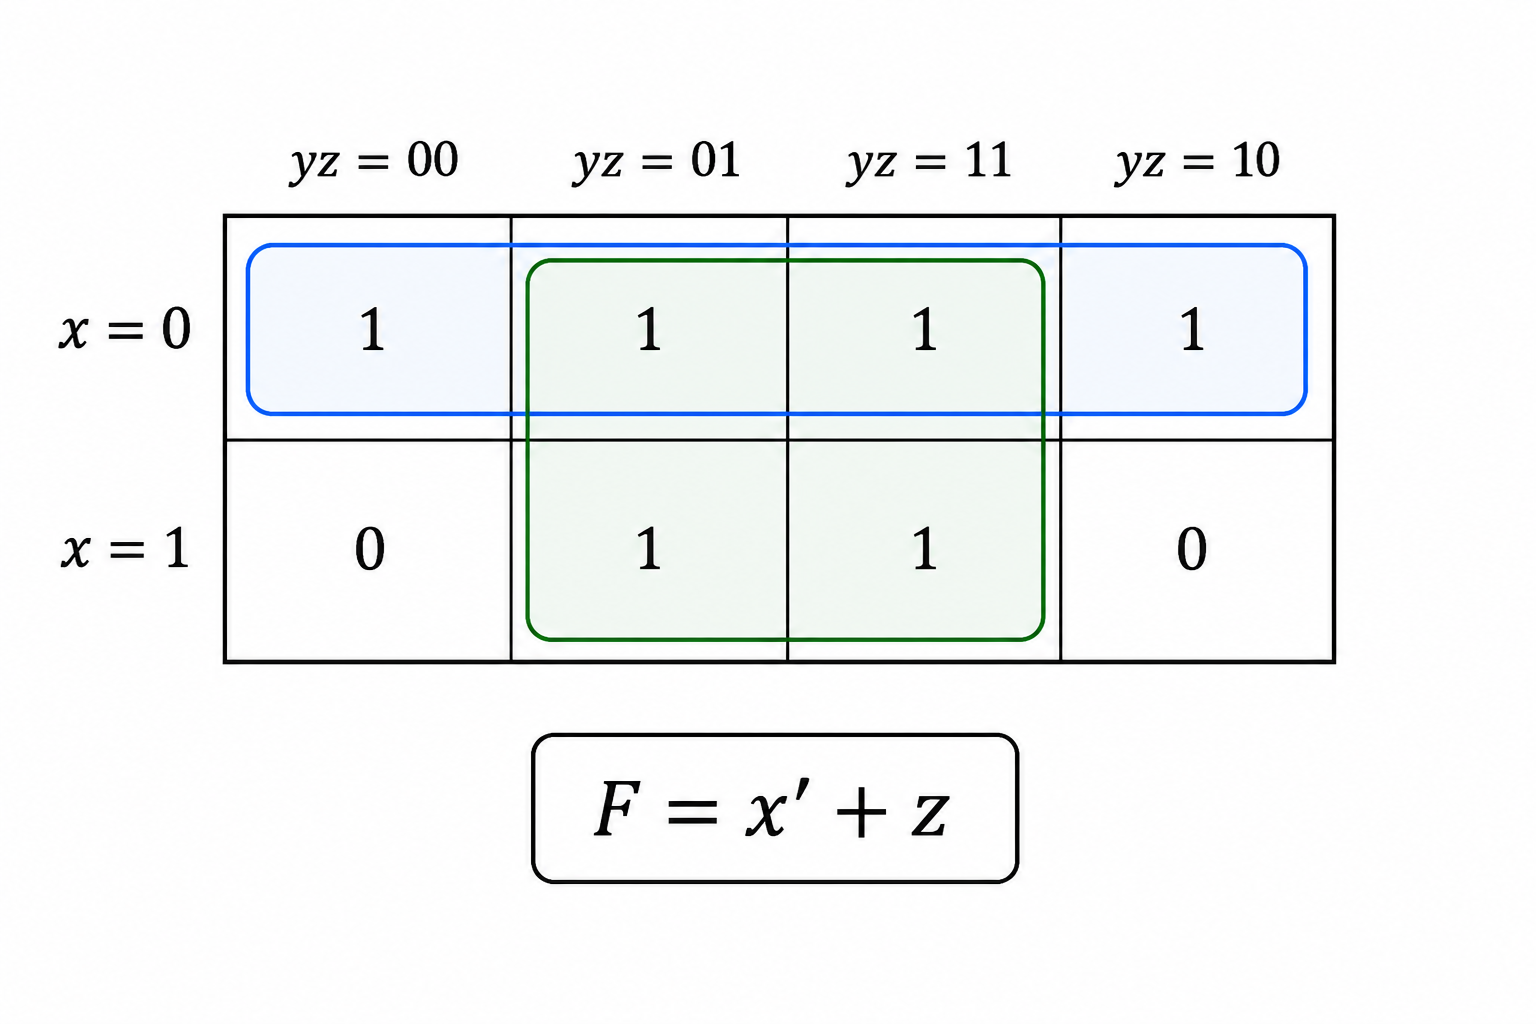
\includegraphics[width=0.82\textwidth]{Figures/png_ready/kmap-grouping-generated.png}
    \caption{การจัดกลุ่มใน K-map}
    \label{fig:kmap-grouping}
\end{figure}

\begin{ex}[การลดรูปด้วยแผนที่คาร์นอ 4 ตัวแปร]
\label{ex:kmap-4var}
ใช้ K-map ลดรูป $f(w, x, y, z) = \sum(0, 1, 2, 3, 4, 6, 8, 9, 12, 14)$

\begin{center}
\begin{tabular}{|c|c|c|c|c|}
\hline
 & $yz = 00$ & $yz = 01$ & $yz = 11$ & $yz = 10$ \\
\hline
$wx = 00$ & 1 & 1 & 1 & 1 \\
\hline
$wx = 01$ & 1 & 0 & 0 & 1 \\
\hline
$wx = 11$ & 1 & 0 & 0 & 1 \\
\hline
$wx = 10$ & 1 & 1 & 0 & 0 \\
\hline
\end{tabular}
\end{center}
\end{ex}
\begin{solution}
\begin{align*}
\{m_0, m_1, m_2, m_3\}\ (\text{แถว } wx = 00) &\Rightarrow w'x'\\
\{m_4, m_6, m_{12}, m_{14}\}\ (\text{แถว } wx = 01 \text{ กับ } wx = 11,\ z = 0) &\Rightarrow xz'\\
\{m_0, m_1, m_8, m_9\}\ (\text{แถวบนสุดกับล่างสุด วนขอบ},\ y = 0) &\Rightarrow x'y'
\end{align*}
$\therefore f = w'x' + xz' + x'y'$ \solhere
\end{solution}

กลุ่ม $\{m_0, m_1, m_8, m_9\}$ ในตัวอย่างข้างต้นเกิดจากการวนขอบในแนวตั้ง คือแถวบนสุดติดกับแถวล่างสุด แผนที่ 4 ตัวแปรวนขอบได้ทั้งสองแนวพร้อมกัน จึงเกิดกรณีพิเศษที่ช่องมุมทั้งสี่รวมเป็นกลุ่มเดียวได้ ทั้งที่มองด้วยตาแล้วดูเหมือนอยู่ห่างกันที่สุดในตาราง

\begin{ex}[การจับกลุ่มวนขอบที่มุมทั้งสี่]
\label{ex:kmap-corner-wrap}
จงใช้แผนที่คาร์นอลดรูป $f(w, x, y, z) = \sum(0, 2, 8, 10)$

\begin{center}
\begin{tabular}{|c|c|c|c|c|}
\hline
 & $yz = 00$ & $yz = 01$ & $yz = 11$ & $yz = 10$ \\
\hline
$wx = 00$ & 1 & 0 & 0 & 1 \\
\hline
$wx = 01$ & 0 & 0 & 0 & 0 \\
\hline
$wx = 11$ & 0 & 0 & 0 & 0 \\
\hline
$wx = 10$ & 1 & 0 & 0 & 1 \\
\hline
\end{tabular}
\end{center}
\end{ex}
\begin{solution}
ทั้งสี่ช่องที่เป็น 1 อยู่ที่มุมทั้งสี่ของตาราง เมื่อวนขอบในแนวตั้ง แถว $wx = 00$ ติดกับแถว $wx = 10$ และเมื่อวนขอบในแนวนอน คอลัมน์ $yz = 00$ ติดกับคอลัมน์ $yz = 10$ ทั้งสี่ช่องจึงติดกันเป็นกลุ่มสี่เหลี่ยมขนาด 4 ช่องกลุ่มเดียว

ตรวจสอบว่าเป็นกลุ่มที่ถูกต้องได้จากรหัสของทั้งสี่มินเทอม
\begin{align*}
m_0 = 0000, \quad m_2 = 0010, \quad m_8 = 1000, \quad m_{10} = 1010
\end{align*}
ตัวแปร $w$ เปลี่ยนค่าและ $y$ เปลี่ยนค่า จึงตัดทั้งคู่ทิ้ง ส่วน $x = 0$ และ $z = 0$ คงที่ทั้งกลุ่ม จึงเขียนเป็นนิเสธทั้งคู่

$\therefore f(w, x, y, z) = x'z'$ \solhere
\end{solution}

\begin{warning}[การจับกลุ่มวนขอบที่มุมทั้งสี่ในแผนที่คาร์นอ]
กับดักที่พบบ่อยคือมองว่าช่องมุมทั้งสี่แยกกันอยู่ แล้วเขียนเป็นสี่พจน์ที่มีสี่ตัวแปรเต็ม คือ $w'x'y'z' + w'x'yz' + wx'y'z' + wx'yz'$ ซึ่งให้ค่าตรงกับฟังก์ชันเดิมก็จริง แต่ใช้ประตูมากกว่าที่จำเป็นหลายเท่า ทั้งที่คำตอบที่ลดรูปแล้วเหลือเพียงพจน์เดียวสองตัวแปร ให้ยึดหลักว่าเซลล์ติดกันคือเซลล์ที่รหัสต่างกันหนึ่งบิต ไม่ใช่เซลล์ที่วาดอยู่ติดกันบนกระดาษ
\end{warning}

\subsection{ค่าไม่สนใจในแผนที่คาร์นอ (Don't Care Conditions)}
\label{sec:dont-care}
ในงานออกแบบระบบดิจิทัลจริง ชุดข้อมูลขาเข้าบางชุดอาจไม่มีทางเกิดขึ้นได้ตามข้อกำหนดการทำงานของระบบ (เช่น เลขฐานสองที่มีค่าเกิน 9 ในระบบเลข BCD) หรือเป็นกรณีที่สัญญาณขาออกไม่มีผลต่อการทำงาน สภาวะดังกล่าวเรียกว่า \textbf{สภาวะไม่สนใจ (Don't Care Conditions)} ซึ่งเขียนแทนด้วยสัญลักษณ์ $d$ หรือ $X$ ในแผนที่คาร์นอ ผู้ออกแบบมีอิสระที่จะกำหนดให้ค่า $d$ เป็น 1 (หากช่วยขยายกลุ่มให้ใหญ่ขึ้นเพื่อลดรูปตัวแปร) หรือกำหนดให้เป็น 0 (หากไม่ต้องการนำมารวมกลุ่ม) เพื่อให้ได้วงจรที่เรียบง่ายและประหยัดที่สุด~\parencite{mano2018digital}

\begin{principle}[การใช้ค่าไม่สนใจในการจับกลุ่ม]
\label{prin:dont-care}
\index{ค่าไม่สนใจ}
เขียนสัญลักษณ์ $d$ ลงในช่องที่เป็นค่าไม่สนใจ แล้วปฏิบัติกับช่องเหล่านั้นตามกฎต่อไปนี้

\begin{enumerate}
    \item ช่อง $d$ \textbf{รวมเข้ากลุ่มได้} เสมือนเป็น 1 ถ้าการรวมนั้นทำให้กลุ่มที่จำเป็นอยู่แล้วขยายใหญ่ขึ้น
    \item ช่อง $d$ \textbf{ไม่ใช่ช่องที่ต้องถูกคลุม} ต่างจากช่องที่เป็น 1 ตามกฎข้อ 5 ใน~\autoref{prin:kmap-rules}
    \item จึง \textbf{ห้ามสร้างกลุ่มขึ้นมาเพื่อคลุมช่อง $d$ โดยเฉพาะ} เพราะจะได้พจน์เพิ่มโดยไม่ได้ประโยชน์
\end{enumerate}

สรุปเป็นเกณฑ์เดียวได้ว่า ตั้ง $d$ เป็น 1 เมื่อมันช่วยขยายกลุ่มที่ต้องมีอยู่แล้ว และตั้งเป็น 0 ในกรณีอื่นทั้งหมด ข้อผิดพลาดที่พบบ่อยคือเข้าใจว่าต้องตั้ง $d$ ทุกช่องเป็น 1 ซึ่งมักทำให้ได้นิพจน์ที่ยาวกว่าเดิม
\end{principle}

\begin{ex}[การลดรูปด้วยค่าไม่สนใจในวงจรตรวจเลขรหัสบีซีดี]
\label{ex:kmap-dont-care}
วงจรหนึ่งรับเลขรหัสบีซีดี (BCD) ขนาด 4 บิต $wxyz$ ซึ่งใช้แทนเลขโดดฐานสิบ 0 ถึง 9 เท่านั้น รหัส 1010 ถึง 1111 จึงไม่มีทางเกิดขึ้น จงออกแบบฟังก์ชัน $f$ ที่ให้ผลลัพธ์เป็น 1 เมื่อเลขโดดที่รับเข้ามามีค่าตั้งแต่ 5 ขึ้นไป นั่นคือ $f = \sum m(5, 6, 7, 8, 9) + d(10, 11, 12, 13, 14, 15)$

\begin{center}
\begin{tabular}{|c|c|c|c|c|}
\hline
 & $yz = 00$ & $yz = 01$ & $yz = 11$ & $yz = 10$ \\
\hline
$wx = 00$ & 0 & 0 & 0 & 0 \\
\hline
$wx = 01$ & 0 & 1 & 1 & 1 \\
\hline
$wx = 11$ & $d$ & $d$ & $d$ & $d$ \\
\hline
$wx = 10$ & 1 & 1 & $d$ & $d$ \\
\hline
\end{tabular}
\end{center}
\end{ex}
\begin{solution}
จับกลุ่มโดยดึงช่อง $d$ เข้ามาช่วยขยายกลุ่ม
\begin{align*}
\{m_8, m_9, m_{10}, m_{11}, m_{12}, m_{13}, m_{14}, m_{15}\}\ (\text{สองแถวล่าง},\ w = 1) &\Rightarrow w\\
\{m_5, m_7, m_{13}, m_{15}\}\ (\text{คอลัมน์ } yz = 01, 11 \text{ ที่ } x = 1) &\Rightarrow xz\\
\{m_6, m_7, m_{14}, m_{15}\}\ (\text{คอลัมน์ } yz = 11, 10 \text{ ที่ } x = 1) &\Rightarrow xy
\end{align*}
ทั้งสามกลุ่มคลุมช่องที่เป็น 1 ครบทั้ง $m_5, m_6, m_7, m_8, m_9$ แล้ว

$\therefore f(w, x, y, z) = w + xy + xz$ \solhere

เปรียบเทียบกับกรณีที่ไม่ใช้ค่าไม่สนใจ คือบังคับให้ช่อง $d$ ทุกช่องเป็น 0 จะจับกลุ่มได้เพียงกลุ่มละ 2 ช่อง ได้ผลลัพธ์เป็น $w x' y' + w' x z + w' x y$ ซึ่งถูกต้องเช่นกันแต่ใช้ตัวแปรรวม 9 ตัวเทียบกับ 5 ตัว การใช้ค่าไม่สนใจจึงลดขนาดวงจรลงได้อย่างมีนัยสำคัญ
\end{solution}

\section{การประยุกต์ในวงจรดิจิทัล}
\label{sec:boolean-applications}

พีชคณิตบูลีนเป็นรากฐานทางทฤษฎีของการออกแบบวงจรดิจิทัล ทุกกระบวนการประมวลผลและการคำนวณในระบบคอมพิวเตอร์สมัยใหม่ ล้วนถูกแปลงเป็นการดำเนินการทางตรรกศาสตร์บนสัญญาณไฟฟ้า 2 ระดับ ($0$ และ $1$) การเข้าใจความสัมพันธ์ระหว่างนิพจน์บูลีนกับโครงสร้างวงจรฮาร์ดแวร์จริง จึงเป็นทักษะที่จำเป็นในการทำความเข้าใจสถาปัตยกรรมคอมพิวเตอร์ กระบวนการออกแบบวงจรดิจิทัลจะเริ่มต้นจากการวิเคราะห์ข้อกำหนดของระบบ แปลงเป็นฟังก์ชันบูลีน ดำเนินการลดรูปนิพจน์ให้กะทัดรัดที่สุด และสังเคราะห์ออกมาเป็นวงจรที่ประกอบด้วยลอจิกเกต (Logic Gates)~\parencite{gersting2014structures}

\subsection{ประตูตรรกะ (Logic Gates)}
ลอจิกเกต (Logic Gates) เป็นอุปกรณ์อิเล็กทรอนิกส์พื้นฐานที่ทำหน้าที่ประมวลผลสัญญาณตามการดำเนินการบูลีนในระดับฮาร์ดแวร์ โดยรับระดับแรงดันไฟฟ้าที่แทนค่า $0$ และ $1$ ทางช่องสัญญาณขาเข้า และส่งสัญญาณผลลัพธ์ขาออกตามตารางค่าความจริงของฟังก์ชันนั้น ๆ การแปลงนิพจน์บูลีนเป็นวงจรจริงสามารถทำได้โดยแทนตัวดำเนินการแต่ละตัวด้วยลอจิกเกตที่สอดคล้องกัน โดยลอจิกเกตพื้นฐานที่สำคัญมีดังนี้~\parencite{wakerly2018digital}


\begin{definition}[ประเภทของประตูตรรกะ]
\index{ประตูตรรกะ!ประเภท}
ประเภทของประตูตรรกะพื้นฐาน ได้แก่
\begin{enumerate}
    \item NOT Gate (Inverter) แสดงผล $a'$
    \item AND Gate แสดงผล $a \cdot b$
    \item OR Gate แสดงผล $a + b$
    \item NAND Gate แสดงผล $(a \cdot b)'$
    \item NOR Gate แสดงผล $(a + b)'$
    \item XOR Gate แสดงผล $a \oplus b = a b' + a' b$
    \item XNOR Gate แสดงผล $(a \oplus b)' = a b + a' b'$
\end{enumerate}
\end{definition}

\begin{principle}[NAND Gate ในฐานะเกตสากล (Universal Gate)]
\index{ประตูตรรกะ!NAND Gate}
\textbf{NAND Gate} เป็นเกตสากล (Universal Gate) เนื่องจากสามารถนำมาต่อเชื่อมเพื่อสร้างเกตตรรกะพื้นฐานอื่น ๆ ได้ทั้งหมด โดย NAND Gate ให้ผลลัพธ์การทำงานคือ $Y = (a \cdot b)' = \overline{a \cdot b}$

ค่าผลลัพธ์ในทุกกรณีของสัญญาณอินพุต $(a, b)$ แสดงไว้ในตารางที่~\ref{tab:nand-nor-truth} จุดที่ควรสังเกตคือ NAND ให้ผลเป็น 0 เพียงกรณีเดียว คือเมื่ออินพุตทั้งสองเป็น 1 ซึ่งตรงข้ามกับ AND ทุกแถวพอดี

การสร้างประตูตรรกะพื้นฐานจากประตู NAND เพียงอย่างเดียวทำได้ดังนี้
\begin{enumerate}[label=\textbf{\arabic*.},leftmargin=1.5em,itemsep=0.4em]
    \item \textbf{การสร้างประตู NOT จาก NAND} เมื่อป้อนสัญญาณเข้าเดียวกันทั้งสองช่อง $(a, a)$ จะได้
    \[ a' = (a \cdot a)' \]
    \item \textbf{การสร้าง AND Gate จาก NAND:} นำผลลัพธ์ของ NAND Gate มาผ่าน NOT Gate (NAND ที่ป้อนอินพุตซ้ำ) ได้ว่า
    \[ a \cdot b = ((a \cdot b)')' \]
    \item \textbf{การสร้างประตู OR จาก NAND} ใช้กฎเดอมอร์แกนร่วมกับการนิเสธสัญญาณเข้าแต่ละตัว
    \[ a + b = (a' \cdot b')' = ((a \cdot a)' \cdot (b \cdot b)')' \]
\end{enumerate}
\end{principle}

\begin{principle}[NOR Gate ในฐานะเกตสากล (Universal Gate)]
\index{ประตูตรรกะ!NOR Gate}
\textbf{NOR Gate} เป็นเกตสากล (Universal Gate) เช่นเดียวกับ NAND Gate เนื่องจากสามารถนำมาต่อเพื่อสร้างเกตตรรกะอื่น ๆ ได้ทั้งหมด โดย NOR Gate ให้ผลลัพธ์การทำงานคือ $Y = (a + b)'$

ค่าผลลัพธ์ในทุกกรณีแสดงไว้ในตารางที่~\ref{tab:nand-nor-truth} เช่นเดียวกัน โดย NOR ให้ผลเป็น 1 เพียงกรณีเดียว คือเมื่ออินพุตทั้งสองเป็น 0 ซึ่งตรงข้ามกับ OR ทุกแถวพอดี

การสร้างประตูตรรกะพื้นฐานจากประตู NOR เพียงอย่างเดียวทำได้ดังนี้
\begin{enumerate}[label=\textbf{\arabic*.},leftmargin=1.5em,itemsep=0.4em]
    \item \textbf{การสร้างประตู NOT จาก NOR} เมื่อป้อนสัญญาณเข้าเดียวกันทั้งสองช่อง $(a, a)$ จะได้
    \[ a' = (a + a)' \]
    \item \textbf{การสร้าง OR Gate จาก NOR:} นำผลลัพธ์ของ NOR Gate มาผ่าน NOT Gate (NOR ที่ป้อนอินพุตซ้ำ) ได้ว่า
    \[ a + b = ((a + b)')' \]
    \item \textbf{การสร้างประตู AND จาก NOR} ใช้กฎเดอมอร์แกนร่วมกับการนิเสธสัญญาณเข้าแต่ละตัว
    \[ a \cdot b = (a' + b')' = ((a + a)' + (b + b)')' \]
\end{enumerate}
\end{principle}

\begin{table}[H]
    \centering
    \caption{ตารางค่าความจริงของ NAND และ NOR เทียบกับ AND และ OR}
    \label{tab:nand-nor-truth}
    \begin{tabular}{|c|c|c|c|c|c|}
        \hline
        $a$ & $b$ & $a \cdot b$ & $(a \cdot b)'$ (NAND) & $a + b$ & $(a + b)'$ (NOR) \\ \hline
        0 & 0 & 0 & 1 & 0 & 1 \\ \hline
        0 & 1 & 0 & 1 & 1 & 0 \\ \hline
        1 & 0 & 0 & 1 & 1 & 0 \\ \hline
        1 & 1 & 1 & 0 & 1 & 0 \\ \hline
    \end{tabular}
\end{table}

ตารางที่~\ref{tab:nand-nor-truth} วางคอลัมน์ของ AND และ OR ไว้ข้างคอลัมน์ของ NAND และ NOR เพื่อให้เห็นว่าเกตทั้งสองคู่ให้ผลตรงข้ามกันทุกแถว เหตุที่เกตทั้งสองสร้างเกตอื่นได้ทั้งหมดก็เพราะรวมการนิเสธไว้ในตัวเองแล้ว จึงไม่ต้องอาศัย NOT Gate แยกต่างหาก ส่วนสัญลักษณ์และการต่อวงจรของเกตสากลทั้งสองแสดงในรูปที่~\ref{fig:universal-gates}

\begin{figure}[H]
    \centering
    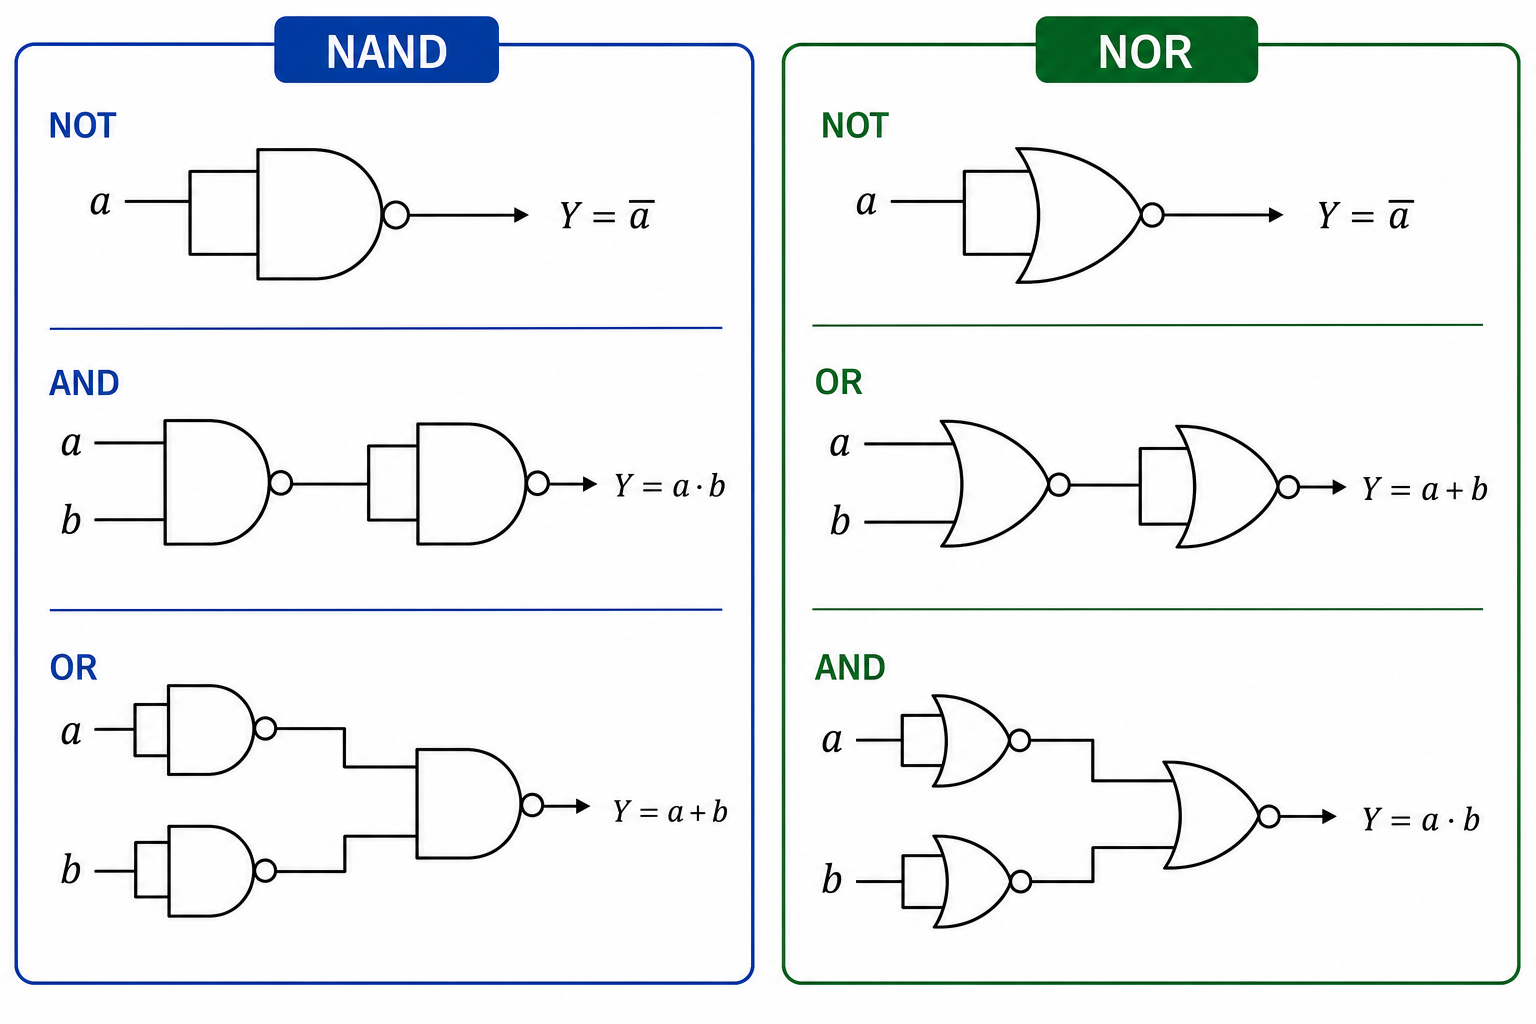
\includegraphics[width=0.82\textwidth]{Figures/png_ready/universal-gates-generated.png}
    \caption{เกตสากล NAND และ NOR}
    \label{fig:universal-gates}
\end{figure}

\begin{ex}[การวาดวงจรจากนิพจน์บูลีน]
\label{ex:draw-circuit}
จงอธิบายลำดับการต่อประตูตรรกะเพื่อสร้างวงจรของ $f(x, y, z) = x y + x' z$ พร้อมนับจำนวนประตูแต่ละชนิดที่ใช้
\end{ex}
\begin{solution}
\begin{align*}
x &\xrightarrow{\text{NOT}} x'\\
(x, y) &\xrightarrow{\text{AND}} xy, \qquad (x', z) \xrightarrow{\text{AND}} x'z\\
(xy, x'z) &\xrightarrow{\text{OR}} xy + x'z = f
\end{align*}

$\therefore$ วงจรใช้ประตู NOT 1 ตัว ประตู AND 2 ตัว และประตู OR 1 ตัว \solhere
\end{solution}

\begin{ex}[การลดรูปก่อนวาดวงจร]
\label{ex:simplify-then-draw}
ลดรูปและวาดวงจรสำหรับ $f(a, b, c) = (a + b) \cdot (a + c)$
\end{ex}
\begin{solution}
\begin{align*}
f &= (a + b)(a + c)\\
&= a + bc \quad \text{(Distributive)}
\end{align*}
วงจร $(b,c) \xrightarrow{\text{AND}} bc$ แล้ว $(a, bc) \xrightarrow{\text{OR}} a + bc$ ใช้ประตู AND 1 ตัวกับประตู OR 1 ตัว จากเดิมที่ต้องใช้ประตู OR 2 ตัวกับประตู AND 1 ตัว

$\therefore$ การลดรูปช่วยลดจำนวนประตูจาก 3 ตัวเหลือ 2 ตัว \solhere
\end{solution}

\subsection{การออกแบบวงจรเชิงผสม (Combinational Circuit)}
วงจรเชิงผสม (Combinational Logic Circuits) คือ วงจรดิจิทัลที่สัญญาณขาออกขึ้นอยู่กับค่าของสัญญาณขาเข้า ณ ขณะเวลาปัจจุบันเท่านั้น โดยไม่มีหน่วยความจำและไม่ขึ้นกับสถานะในอดีต การออกแบบวงจรเชิงผสมประกอบด้วยขั้นตอนการแปลงข้อกำหนดของระบบเป็นตารางค่าความจริง การเขียนฟังก์ชันบูลีนในรูปแบบบัญญัติ การลดรูปนิพจน์ด้วยแผนที่คาร์นอ และการต่อวงจรด้วยลอจิกเกตตามลำดับ~\parencite{wakerly2018digital}

\begin{ex}[การออกแบบวงจรตรวจสอบจำนวนคู่]
\label{ex:even-detector}
ออกแบบวงจรที่ตรวจสอบว่าจำนวน 3-bit เป็นเลขคู่ (even)
\end{ex}
\begin{solution}
ให้บิต $z$ เป็นบิตต่ำสุด (LSB); จำนวนเป็นเลขคู่ ก็ต่อเมื่อ $z = 0$ ได้ minterms $m_0, m_2, m_4, m_6$
\begin{align*}
f(x, y, z) &= x'y'z' + x'yz' + xy'z' + xyz'\\
&= z' \quad (\text{ตรวจสอบบิตต่ำสุด})
\end{align*}

$\therefore$ วงจรตรวจสอบจำนวนคู่ใช้เพียงประตู NOT ตัวเดียวที่บิตต่ำสุด เพราะจำนวนคู่คือจำนวนที่บิตต่ำสุดเป็น 0 \solhere
\end{solution}

\subsection{การสร้างวงจรสองระดับ (Two-level Realization)}
\label{sec:two-level}
การสร้างวงจรดิจิทัลแบบ 2 ระดับ (Two-Level Realization) เป็นการจัดวางลอจิกเกตหลักเพียง 2 ชั้นก่อนส่งสัญญาณถึงขาออก (ไม่นับอินเวอร์เตอร์ที่ใช้กลับค่าสัญญาณตัวแปร) นิพจน์ในรูปแบบ SOP และ POS สามารถแปลงเป็นวงจร 2 ระดับได้โดยตรง โครงสร้างนี้มีจุดเด่นด้านความเร็วในการทำงาน เนื่องจากสัญญาณจะผ่านเกตเพียง 2 ชั้น ทำให้มีเวลาหน่วงการแพร่สัญญาณที่ต่ำและคงที่~\parencite{wakerly2018digital}

\begin{principle}[การสร้างวงจรสองระดับ]
\textbf{Two-level Realization:}
\begin{enumerate}
    \item SOP (Sum of Products) AND gates ระดับแรก แล้ว OR gate ระดับที่สอง
    \item POS (Product of Sums) OR gates ระดับแรก แล้ว AND gate ระดับที่สอง
\end{enumerate}
\end{principle}

\begin{ex}[การสร้างวงจรสองระดับแบบ SOP]
\label{ex:two-level-sop}
จงอธิบายการสร้างวงจรสองระดับแบบ SOP ของ $f(x, y, z) = y' + x y + x' y' z$ พร้อมระบุว่าความหน่วงเวลาของวงจรขึ้นกับสิ่งใด
\end{ex}
\begin{solution}
ระดับแรก $(x,y) \xrightarrow{\text{AND}} xy$ และ $(x',y',z) \xrightarrow{\text{AND}} x'y'z$ (ใช้ NOT สร้าง $x', y'$); ระดับที่สอง $(y',\ xy,\ x'y'z) \xrightarrow{\text{OR}} f$

$\therefore$ วงจรสองระดับนี้มีความหน่วงเวลาคงที่ ไม่ขึ้นกับจำนวนพจน์ เพราะทุกสัญญาณผ่านประตูเพียงสองชั้น \solhere
\end{solution}

\subsection{วงจรบวกครึ่งและวงจรบวกเต็ม (Half Adder and Full Adder)}
\label{sec:adders}
วงจรบวกเลขฐานสอง (Binary Adders) เป็นตัวอย่างคลาสสิกของการนำพีชคณิตบูลีนไปสร้างเป็นวงจรคำนวณในหน่วยประมวลผลกลาง โดย \textbf{วงจรบวกครึ่ง (Half Adder)} รับข้อมูลขาเข้า 2 บิตเพื่อคำนวณผลบวก ($S$) และบิตทด ($C$) ในขณะที่ \textbf{วงจรบวกเต็ม (Full Adder)} รับสัญญาณขาเข้า 3 บิต ซึ่งรวมบิตทดรับเข้า ($C_{in}$) จากหลักก่อนหน้า ทำให้สามารถนำวงจรบวกเต็มมาต่ออนุกรมกันเป็นชุดเพื่อบวกเลขฐานสองขนาดหลายบิต (Multi-bit Adder) ภายในหน่วยคำนวณและตรรกะ (ALU) ได้อย่างสมบูรณ์~\parencite{wakerly2018digital}

\begin{ex}[การออกแบบวงจรบวกครึ่ง]
\label{ex:half-adder}
ออกแบบวงจรบวกครึ่ง (Half Adder)
\end{ex}
\begin{solution}
Half Adder รับ 2 บิต $x, y$
\begin{align*}
S &= x \oplus y = x y' + x' y\\
C &= x \cdot y
\end{align*}

$\therefore$ วงจรบวกครึ่งใช้ประตู XOR 1 ตัวสำหรับผลบวก และประตู AND 1 ตัวสำหรับตัวทด \solhere
\end{solution}

\begin{ex}[การออกแบบวงจรบวกเต็ม]
\label{ex:full-adder}
ออกแบบ Full Adder
\end{ex}
\begin{solution}
Full Adder รับ 3 บิต $x, y, z_{in}$
\begin{align*}
S &= x \oplus y \oplus z_{in}\\
C_{out} &= x y + x z_{in} + y z_{in}
\end{align*}

$\therefore$ วงจรบวกเต็มต่างจากวงจรบวกครึ่งตรงที่รับตัวทดเข้ามาด้วย จึงนำไปต่อกันเป็นชุดสำหรับเลขหลายบิตได้ \solhere
\end{solution}

\subsection{สมมูลของพีชคณิตบูลีน (Boolean Algebra Equivalence)}
\label{sec:boolean-equivalence}
กฎที่ศึกษามาตลอดบทนี้มีจำนวนมากจนจดจำได้ยาก การรวบรวมไว้ในที่เดียวช่วยให้เปรียบเทียบและเลือกใช้ได้สะดวกขณะลดรูปนิพจน์ ตารางต่อไปนี้สรุปกฎทั้งหมดพร้อมชื่อเรียกมาตรฐาน โดยจัดคู่กฎที่เป็นคู่ทวิภาค (Dual) ไว้ในแถวเดียวกัน ซึ่งได้จากการสลับ AND กับ OR และสลับ 0 กับ 1 พร้อมกัน~\parencite{mano2018digital}

ตารางที่~\ref{tab:boolean-op-summary} สรุปเงื่อนไขที่ทำให้การดำเนินการพื้นฐานแต่ละตัวให้ผลลัพธ์เป็น 1 หรือ 0 และตารางที่~\ref{tab:boolean-identities} สรุปกฎทั้งหมดโดยจัดคู่ทวิภาคไว้ในแถวเดียวกัน

\begin{table}[!htb]
\centering
\caption{เงื่อนไขที่ทำให้การดำเนินการพื้นฐานให้ผลลัพธ์เป็น 1 และ 0}
\label{tab:boolean-op-summary}
\begin{tabular}{|c|c|c|c|}
\hline
การดำเนินการ & สัญลักษณ์ & ผลลัพธ์เป็น 1 เมื่อ & ผลลัพธ์เป็น 0 เมื่อ \\
\hline
OR & $+$ & มีอินพุตอย่างน้อยหนึ่งตัวเป็น 1 & อินพุตทุกตัวเป็น 0 \\
\hline
AND & $\cdot$ & อินพุตทุกตัวเป็น 1 & มีอินพุตอย่างน้อยหนึ่งตัวเป็น 0 \\
\hline
NOT & $'$ & อินพุตเป็น 0 & อินพุตเป็น 1 \\
\hline
\end{tabular}
\end{table}

\begin{table}[!htb]
\centering
\caption{สรุปกฎของพีชคณิตบูลีน โดยกฎในแถวเดียวกันเป็นคู่ทวิภาคของกันและกัน}
\label{tab:boolean-identities}
\begin{tabular}{|c|c|c|}
\hline
กฎทางพีชคณิต & รูปแบบ OR & รูปแบบ AND \\
\hline
กฎเอกลักษณ์ (Identity) & $x + 0 = x$ & $x \cdot 1 = x$ \\
\hline
กฎครอบงำ (Domination) & $x + 1 = 1$ & $x \cdot 0 = 0$ \\
\hline
กฎนิจพล (Idempotent) & $x + x = x$ & $x \cdot x = x$ \\
\hline
กฎคอมพลีเมนต์ (Complement) & $x + x' = 1$ & $x \cdot x' = 0$ \\
\hline
กฎการสลับที่ (Commutative) & $x + y = y + x$ & $x \cdot y = y \cdot x$ \\
\hline
กฎการเปลี่ยนหมู่ (Associative) & $(x + y) + z = x + (y + z)$ & $(x \cdot y) \cdot z = x \cdot (y \cdot z)$ \\
\hline
กฎการแจกแจง (Distributive) & $x + yz = (x + y)(x + z)$ & $x(y + z) = xy + xz$ \\
\hline
กฎการดูดกลืน (Absorption) & $x + xy = x$ & $x(x + y) = x$ \\
\hline
กฎเดอมอร์แกน (De Morgan's) & $(x + y)' = x' y'$ & $(xy)' = x' + y'$ \\
\hline
\end{tabular}
\end{table}

\section{ตัวอย่างในวิทยาการคอมพิวเตอร์}
\label{sec:computer-science-examples}

พีชคณิตบูลีนมีการประยุกต์ใช้อย่างกว้างขวางในวิทยาการคอมพิวเตอร์ นอกเหนือจากการออกแบบวงจรดิจิทัลแล้ว หลักการทางบูลีนยังปรากฏอย่างเด่นชัดในโครงสร้างการตัดสินใจของภาษาโปรแกรม การเขียนคำสั่งสืบค้นในระบบฐานข้อมูล ขั้นตอนวิธีการเข้ารหัสลับ และการออกแบบสถาปัตยกรรมระบบคอมพิวเตอร์ การศึกษาตัวอย่างการประยุกต์ใช้งานเหล่านี้จะช่วยให้ผู้เรียนเชื่อมโยงความรู้เชิงทฤษฎีเข้ากับการปฏิบัติการทางวิศวกรรมคอมพิวเตอร์ได้อย่างเป็นรูปธรรม~\parencite{gersting2014structures}

\subsection{การใช้แผนที่คาร์นอในงานออกแบบจริง}
หัวข้อย่อยนี้นำเทคนิคแผนที่คาร์นอที่ได้ศึกษามาประยุกต์ใช้กับโจทย์การออกแบบวงจรจริง ซึ่งช่วยให้สามารถลดทอนความซับซ้อนของวงจรได้อย่างมีประสิทธิภาพก่อนการประกอบวงจรฮาร์ดแวร์~\parencite{roth2021logic}

\begin{ex}[การใช้แผนที่คาร์นอในงานออกแบบจริง]
\label{ex:kmap-real-design}
ลดรูปฟังก์ชันบูลีน $F(x,y,z) = \sum(0,1,2,3,5,7)$ โดยใช้ K-map

K-map สำหรับ 3 ตัวแปร ดังนี้


\begin{center}
\begin{tabular}{c|c|c|c|c}
\hline
 & $yz=00$ & $yz=01$ & $yz=11$ & $yz=10$ \\
\hline
$x=0$ & 1 & 1 & 1 & 1 \\
\hline
$x=1$ & 0 & 1 & 1 & 0 \\
\hline
\end{tabular}
\end{center}
\end{ex}
\begin{solution}
\begin{align*}
\{m_0, m_1, m_2, m_3\}\ (\text{แถว } x = 0) &\Rightarrow x'\\
\{m_1, m_3, m_5, m_7\}\ (\text{สองคอลัมน์ } z = 1) &\Rightarrow z
\end{align*}
$\therefore F = x' + z$ \solhere
\end{solution}


\subsection{ตัวอย่างการสร้าง AND จาก NAND}
จากสมบัติของเกตสากล (Universal Gate) ที่ระบุว่าเกต NAND สามารถนำมาต่อเพื่อสร้างการทำงานของลอจิกเกตพื้นฐานอื่น ๆ ได้อย่างสมบูรณ์ ตัวอย่างนี้จะแสดงขั้นตอนการสังเคราะห์เกต AND โดยใช้เกต NAND เพียง 2 ตัว ซึ่งเป็นเทคนิคที่ใช้จริงในสายการผลิตชิปวงจรรวม (Integrated Circuit: IC) เพื่อลดความหลากหลายของชนิดเกตในกระบวนการผลิต~\parencite{mano2018digital}

\begin{ex}[การสร้างประตู AND จากประตู NAND]
\label{ex:and-from-nand}
จงแสดงวิธีสร้างประตู AND ที่ให้ผลลัพธ์ $Y = A \cdot B$ โดยใช้ประตู NAND เพียงชนิดเดียว พร้อมระบุจำนวนประตูที่ใช้
\end{ex}
\begin{solution}
\begin{align*}
\text{NOT จาก NAND}\quad (A \cdot A)' &= A'\\
\text{AND จาก NAND สองตัว}\quad ((AB)')' &= AB
\end{align*}

$\therefore$ สร้างประตู AND ได้ด้วยประตู NAND 2 ตัว คือตัวแรกให้ $(AB)'$ และตัวที่สองทำหน้าที่เป็นตัวนิเสธโดยป้อนสัญญาณเดียวกันเข้าทั้งสองขา ประตู NAND จึงสร้างประตูพื้นฐานได้ทุกชนิด และเรียกว่าประตูสากล \solhere
\end{solution}

\subsection{การต่อวงจรบวกเป็นชุดสำหรับเลขหลายบิต}
วงจรบวกครึ่งและวงจรบวกเต็มสามารถนำมาต่อเรียงกันเป็นวงจรบวกแบบขนาน (Ripple Carry Adder) สำหรับคำนวณเลขฐานสองขนาดหลายบิต โดยส่งบิตทดขาออกจากหลักหนึ่งไปเป็นบิตทดขาเข้าของหลักถัดไป โครงสร้างนี้ทำหน้าที่เป็นแกนหลักในหน่วยคำนวณและตรรกะ (ALU) ของหน่วยประมวลผลกลาง~\parencite{wakerly2018digital} ตัวอย่างต่อไปนี้แสดงการสังเคราะห์วงจรบวกเต็มโดยอาศัยวงจรบวกครึ่ง 2 ชุดร่วมกับเกต OR 1 ตัว ดังแสดงการเปรียบเทียบโครงสร้างในรูปที่~\ref{fig:adders-comparison}

\begin{figure}[H]
    \centering
    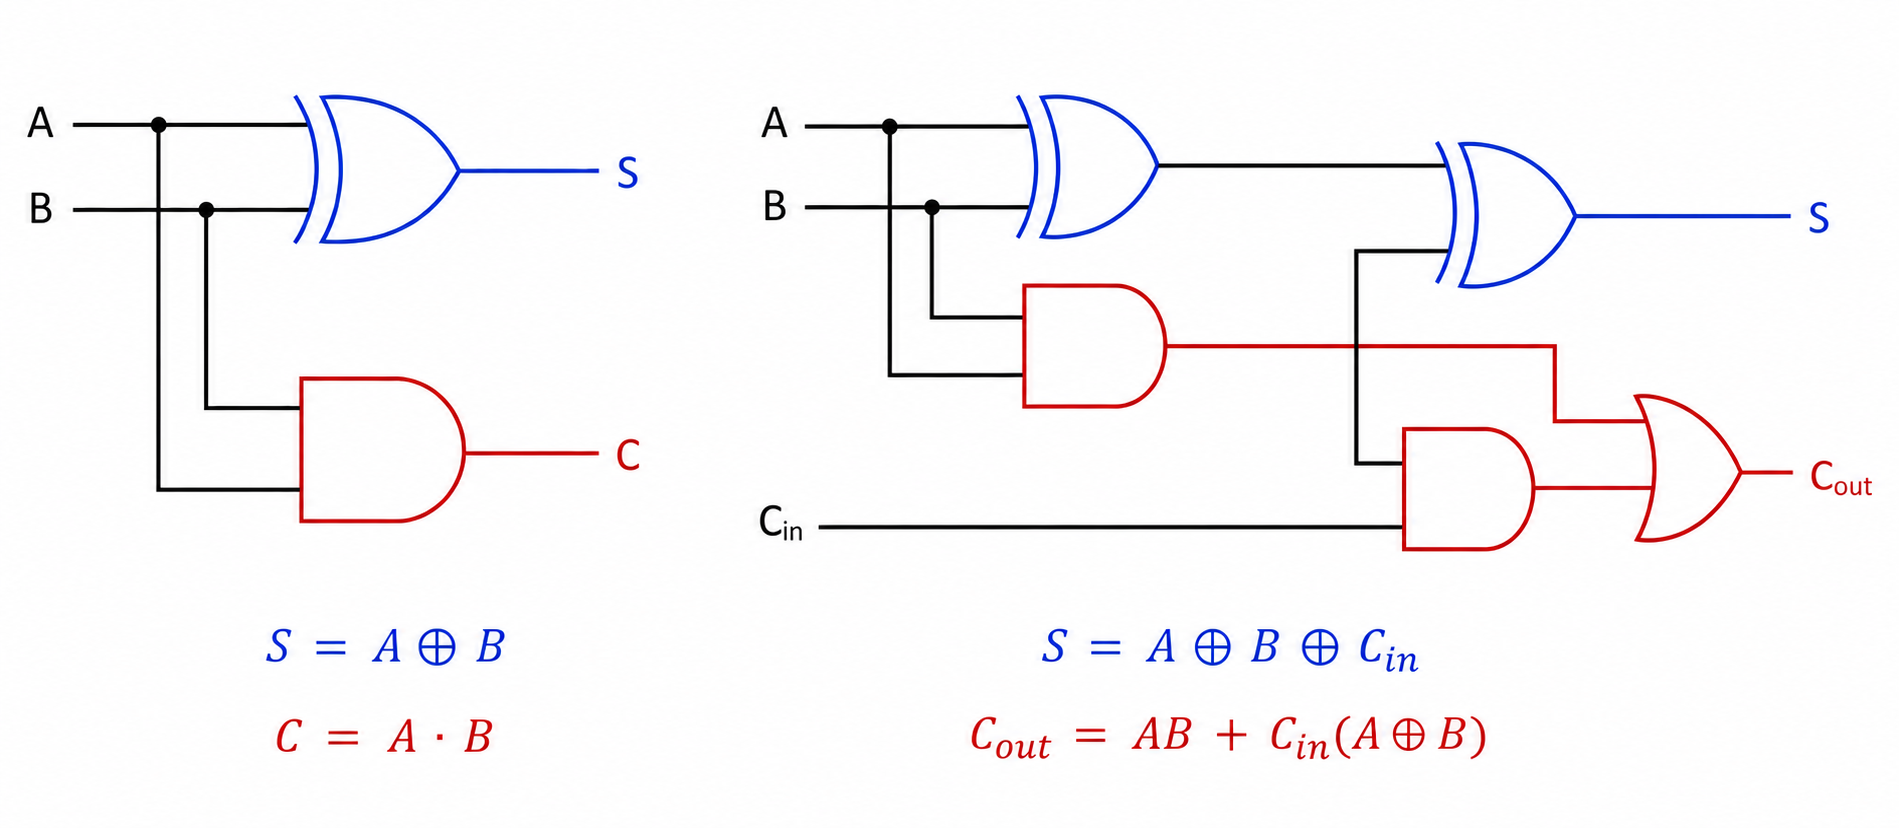
\includegraphics[width=0.82\textwidth]{Figures/png_ready/adders-comparison-generated.png}
    \caption{Half Adder และ Full Adder}
    \label{fig:adders-comparison}
\end{figure}

\begin{ex}[การต่อวงจรบวกครึ่งเป็นวงจรบวกเต็ม]
\label{ex:full-from-half}
Full Adder จาก Half Adders:

$S = A \oplus B \oplus C_{in}$

$C_{out} = AB + C_{in}(A \oplus B)$

สามารถสร้างได้จาก 2 Half Adders + 1 OR gate
\end{ex}
\begin{solution}
\begin{align*}
\text{HA}_1(A, B):\quad S_1 &= A \oplus B, & C_1 &= AB\\
\text{HA}_2(S_1, C_{in}):\quad S &= S_1 \oplus C_{in} = A \oplus B \oplus C_{in}, & C_2 &= C_{in} S_1\\
\text{OR}(C_1, C_2):\quad C_{out} &= AB + C_{in}(A \oplus B)
\end{align*}

$\therefore$ วงจรบวกเต็มหนึ่งตัวสร้างได้จากวงจรบวกครึ่งสองตัวกับประตู OR หนึ่งตัว \solhere
\end{solution}

\subsection{มัลติเพล็กเซอร์และดีมัลติเพล็กเซอร์ (Multiplexer and Demultiplexer)}
\textbf{มัลติเพล็กเซอร์ (Multiplexer: MUX)} และ \textbf{ดีมัลติเพล็กเซอร์ (Demultiplexer: DEMUX)} เป็นวงจรเชิงผสมที่มีบทบาทสำคัญในการควบคุมเส้นทางข้อมูล โดยมัลติเพล็กเซอร์ทำหน้าที่เลือกสัญญาณจากช่องสัญญาณขาเข้าหลายช่อง ($n$ Inputs) ให้ส่งผ่านออกไปยังช่องสัญญาณขาออกเพียงช่องเดียว (1 Output) ตามการควบคุมของสัญญาณเลือก (Select Lines) ในขณะที่ดีมัลติเพล็กเซอร์จะทำหน้าที่ตรงกันข้าม คือ รับสัญญาณขาเข้า 1 ช่องแล้วกระจายไปยังช่องสัญญาณขาออกช่องใดช่องหนึ่งจากหลายช่อง ทั้งสองวงจรสามารถอธิบายการทำงานและออกแบบด้วยนิพจน์บูลีนได้อย่างสมบูรณ์~\parencite{wakerly2018digital}

\begin{definition}[ตัวเลือกข้อมูล (Multiplexer)]
\index{มัลติเพล็กเซอร์!นิยาม}
มัลติเพล็กเซอร์ (Multiplexer: MUX) เป็นวงจรที่เลือก 1 จาก $n$ inputs ไปยัง 1 output โดยใช้ select lines

สำหรับ 4-to-1 MUX:
$$Y = I_0 \cdot S_1' \cdot S_0' + I_1 \cdot S_1' \cdot S_0 + I_2 \cdot S_1 \cdot S_0' + I_3 \cdot S_1 \cdot S_0$$

\begin{center}
\begin{tabular}{|c|c|c|}
\hline
$S_1$ & $S_0$ & สัญญาณออก (Output) \\
\hline
0 & 0 & $I_0$ \\
\hline
0 & 1 & $I_1$ \\
\hline
1 & 0 & $I_2$ \\
\hline
1 & 1 & $I_3$ \\
\hline
\end{tabular}
\end{center}
\end{definition}

\begin{definition}[ตัวกระจายข้อมูล (Demultiplexer)]
\index{ดีมัลติเพล็กเซอร์!นิยาม}
ดีมัลติเพล็กเซอร์ (Demultiplexer: DEMUX) ทำงานตรงข้ามกับ MUX คือรับ 1 input และส่งไปยัง 1 จาก $n$ outputs
\end{definition}

\subsection{การสร้างเครื่องสถานะจำกัดด้วยตรรกะบูลีน (Finite State Machine)}
\textbf{เครื่องสถานะจำกัด (Finite State Machine: FSM)} เป็นแบบจำลองทางคณิตศาสตร์ของวงจรตรรกะเชิงลำดับ (Sequential Circuits) ซึ่งสัญญาณขาออกจะขึ้นอยู่กับทั้งสัญญาณขาเข้าในปัจจุบันและสถานะของวงจรที่ถูกบันทึกไว้ในหน่วยความจำ (ฟลิปฟลอป) การออกแบบ FSM ด้วยพีชคณิตบูลีนทำได้โดยการเข้ารหัสสถานะ (State Encoding) เป็นเลขฐานสอง แล้วสร้างฟังก์ชันบูลีนเพื่อกำหนดสถานะถัดไป (Next State Logic) และสัญญาณขาออก (Output Logic) ตัวอย่างต่อไปนี้แสดงการออกแบบเครื่องสถานะจำกัดแบบมัวร์ (Moore Machine) ซึ่งค่าสัญญาณขาออกจะขึ้นกับสถานะปัจจุบันเท่านั้น~\parencite{wakerly2018digital}

\begin{ex}[การออกแบบเครื่องสถานะจำกัดตรวจจับลำดับบิต]
\label{ex:fsm-sequence}
พิจารณา Moore FSM ที่ตรวจสอบลำดับบิต ``10'' โดย output เป็น 1 หลังจากอ่านบิต 0 ที่ต่อจากบิต 1 แล้ว ดังนี้


\begin{center}
\begin{tabular}{|c|c|c|c|}
\hline
สถานะปัจจุบัน (State) & สัญญาณเข้า=0 & สัญญาณเข้า=1 & สัญญาณออก (Output) \\
\hline
S0 (เริ่มต้น) & S0 & S1 & 0 \\
\hline
S1 (พบบิต 1) & S2 & S1 & 0 \\
\hline
S2 (พบลำดับ 10) & S0 & S1 & 1 \\
\hline
\end{tabular}
\end{center}

กำหนด state encoding: S0=00, S1=01, S2=10 โดยกำหนดสถานะ 11 เป็นค่าไม่สนใจ

จากตารางสถานะ จะได้สมการสถานะถัดไปและผลลัพธ์ดังนี้
\[
Q_1^+ = Q_0X', \qquad Q_0^+ = X, \qquad Y = Q_1Q_0'
\]

ตัวอย่างเช่น input $11010$ จะเดินสถานะเป็น $S0 \rightarrow S1 \rightarrow S1 \rightarrow S2 \rightarrow S1 \rightarrow S2$ ดังนั้น output หลังอ่านแต่ละบิตคือ $0,0,1,0,1$ โดยค่า 1 เกิดเมื่อเครื่องเข้าสู่ state $S2$
\end{ex}
\begin{solution}
ใช้ตัวแปรสถานะ $Q_1,Q_0$ แทนสามสถานะ จะได้ $Q_1^+=Q_0X'$, $Q_0^+=X$ และ $Y=Q_1Q_0'$ ซึ่งเป็นสมการสำหรับสร้างวงจรสถานะถัดไปและวงจรผลลัพธ์

$\therefore$ เครื่องสถานะจำกัดนี้สร้างได้จากฟลิปฟลอป 2 ตัวกับวงจรตรรกะเชิงผสมที่คำนวณสมการทั้งสาม \solhere
\end{solution}

\sectionbanner{สรุปบทเรียน}
\label{sec:chapter-summary-boolean}
เนื้อหาในบทนี้ได้นำเสนอแนวคิดพื้นฐานเกี่ยวกับพีชคณิตบูลีน $(B, +, \cdot, ', 0, 1)$ และสัจพจน์ที่เกี่ยวข้อง โดยเริ่มต้นจากการดำเนินการทางตรรกะพื้นฐาน ได้แก่ OR ($+$), AND ($\cdot$) และ NOT ($'$) ตลอดจนการดำเนินการ XOR ($\oplus$) พร้อมทั้งแสดงพฤติกรรมการทำงานด้วยตารางค่าความจริง จากนั้นได้ศึกษากฎและเอกลักษณ์ของพีชคณิตบูลีน เช่น กฎเอกลักษณ์ กฎการครอบงำ กฎการนิจพล กฎคอมพลีเมนต์ กฎการสลับที่ กฎการเปลี่ยนหมู่ กฎการแจกแจง กฎการดูดกลืน และกฎเดอมอร์แกน ซึ่งเชื่อมโยงโดยตรงกับหลักการทวิภาค ในส่วนของการสร้างแบบจำลอง ได้นำเสนอการเขียนฟังก์ชันบูลีนในรูปแบบบัญญัติ ทั้งแบบผลบวกของผลคูณ (SOP) และผลคูณของผลบวก (POS) และเทคนิคการลดรูปนิพจน์ด้วยแผนที่คาร์นอ (Karnaugh Map) รวมถึงการจัดการสภาวะไม่สนใจ (Don't Care Conditions) ก่อนจะปิดท้ายด้วยการประยุกต์ใช้ในวงจรดิจิทัล เช่น ลอจิกเกต เกตสากล (NAND และ NOR) วงจรเชิงผสม วงจรบวกเลขฐานสอง (Half Adder และ Full Adder) มัลติเพล็กเซอร์ ดีมัลติเพล็กเซอร์ และเครื่องสถานะจำกัด (FSM)

พีชคณิตบูลีนเป็นพื้นฐานสำหรับการศึกษาทฤษฎีการคำนวณและการออกแบบวงจรดิจิทัล ซึ่งใช้วงจรบูลีนและนิพจน์บูลีนโดยตรง

ความเชื่อมโยงระหว่างพีชคณิตบูลีน ตรรกศาสตร์ และทฤษฎีเซตเป็นสิ่งสำคัญที่แสดงให้เห็นว่าโครงสร้างทางคณิตศาสตร์ต่าง ๆ มีความสัมพันธ์กัน~\parencite{rosen2019discrete}

\clearpage
\sectionbanner{แบบฝึกหัด}
\label{sec:exercises-boolean}

\exercisepart{ส่วนที่ 1 การดำเนินการพื้นฐาน}
\begin{exercise}
จงหาค่าของนิพจน์ต่อไปนี้
\begin{enumerate}
    \item $1 + 0$
    \item $1 \cdot 1$
    \item $0'$
    \item $1' + 0$
    \item $1 \cdot 0 + 1$
    \item $(1 + 0) \cdot 1$
    \item $(1')'$
    \item $1 \cdot 1 + 0 \cdot 1$
\end{enumerate}
\end{exercise}

\begin{exercise}
จงเขียนตารางค่าความจริงของฟังก์ชันต่อไปนี้
\begin{enumerate}
    \item $f(x, y) = x + y'$
    \item $f(x, y) = (x + y)'$
    \item $f(x, y) = x \cdot y + x' \cdot y'$
    \item $f(x, y) = (x \oplus y)'$
\end{enumerate}
\end{exercise}

\begin{exercise}
จงพิจารณาว่าข้อความต่อไปนี้จริงหรือเท็จ พร้อมให้เหตุผล
\begin{enumerate}
    \item $1 + 1 = 2$
    \item $1 \cdot 1 = 1$
    \item $0' = 0$
    \item $(1')' = 1$
    \item $x + 1 = 1$ สำหรับทุก $x$
    \item $x \cdot 0 = x$ สำหรับทุก $x$
\end{enumerate}
\end{exercise}

\exercisepart{ส่วนที่ 2 กฎของพีชคณิตบูลีน}
\begin{exercise}
จงพิสูจน์เอกลักษณ์ต่อไปนี้โดยใช้ตารางค่าความจริง
\begin{enumerate}
    \item $x \cdot (x + y) = x$
    \item $x + x' y = x + y$
    \item $(x + y)(x + z) = x + y z$
\end{enumerate}
\end{exercise}

\begin{exercise}
จงลดรูปนิพจน์ต่อไปนี้โดยใช้กฎของพีชคณิตบูลีนในตารางที่~\ref{tab:boolean-identities}
\begin{enumerate}
    \item $x + x y$
    \item $x \cdot (x' + y)$
    \item $(x + y)(x + y')$
    \item $x y + x y'$
    \item $(x + y)' + x$
    \item $x' y + x y' + x y$
\end{enumerate}
\end{exercise}

\begin{exercise}
จงใช้ทฤษฎีบทคอนเซนซัสตัดพจน์ที่ไม่จำเป็นออกจากนิพจน์ต่อไปนี้ พร้อมระบุว่าพจน์ใดเป็นพจน์คอนเซนซัสและเกิดจากตัวแปรคู่ใด
\begin{enumerate}
    \item $a' b + a c + b c$
    \item $w x + w' y + x y$
    \item $(p + q)(p' + r)(q + r)$
    \item $x y + x' z + y z w$
\end{enumerate}
\end{exercise}

\exercisepart{ส่วนที่ 3 กฎเดอมอร์แกน}
\begin{exercise}
จงพิสูจน์กฎเดอมอร์แกนต่อไปนี้
\begin{enumerate}
    \item $(x + y)' = x' y'$
    \item $(x y)' = x' + y'$
\end{enumerate}
\end{exercise}

\begin{exercise}
จงใช้กฎเดอมอร์แกนเขียนคอมพลีเมนต์ของนิพจน์ต่อไปนี้
\begin{enumerate}
    \item $x y + x' z$
    \item $(x + y + z)(x' y' z')'$
    \item $(a + b)(c + d)$
    \item $a + b c'$
\end{enumerate}
\end{exercise}

\exercisepart{ส่วนที่ 4 ฟังก์ชันบูลีนและรูปแบบบัญญัติ}
\begin{exercise}
จงเขียนตารางค่าความจริงของฟังก์ชันต่อไปนี้
\begin{enumerate}
    \item $f(x, y, z) = x y + y z + x z$
    \item $f(x, y, z) = (x + y)(y + z)(x + z)$
    \item $f(x, y, z) = x \oplus y \oplus z$
\end{enumerate}
\end{exercise}

\begin{exercise}
จงเขียนฟังก์ชันต่อไปนี้ในรูปแบบบัญญัติ SOP (สัญกรณ์ $\sum$)
\begin{enumerate}
    \item $f(x, y) = x + y'$
    \item $f(x, y, z) = x y + x' z$
\end{enumerate}
\end{exercise}

\begin{exercise}
จงเขียนฟังก์ชันต่อไปนี้ในรูปแบบบัญญัติ POS (สัญกรณ์ $\prod$)
\begin{enumerate}
    \item $f(x, y) = x \oplus y$
    \item $f(x, y, z) = (x + y')(x' + z)$
\end{enumerate}
\end{exercise}

\exercisepart{ส่วนที่ 5 แผนที่คาร์นอ}
\begin{exercise}
จงใช้แผนที่คาร์นอลดรูปฟังก์ชันต่อไปนี้
\begin{enumerate}
    \item $f(x, y) = \sum(1, 2, 3)$
    \item $f(x, y) = \sum(0, 1, 2)$
    \item $f(x, y, z) = \sum(0, 2, 4, 6)$
    \item $f(x, y, z) = \sum(1, 3, 5, 7)$
    \item $f(w, x, y, z) = \sum(0, 2, 4, 6, 8, 10, 12, 14)$
\end{enumerate}
\end{exercise}

\begin{exercise}
จงออกแบบวงจรต่อไปนี้ พร้อมเขียนนิพจน์บูลีนของสัญญาณออกทุกตัว
\begin{enumerate}
    \item วงจรบวกครึ่ง โดยเขียนนิพจน์ของทั้งบิตผลบวกและบิตทด
    \item มัลติเพล็กเซอร์ 2-to-1 ที่มีสัญญาณเลือก $s$ และข้อมูลเข้า $d_0, d_1$
    \item วงจรที่ให้ผลลัพธ์เป็น 1 เมื่อข้อมูลเข้า 3 บิตมีบิตที่เป็น 1 อยู่ 2 บิตพอดี
\end{enumerate}
\end{exercise}

\answerkeyhead
\label{sec:exercises-solutions}

\exercisepart{เฉลยส่วนที่ 1 การดำเนินการพื้นฐาน}
\begin{enumerate}[series=anskey,label={},leftmargin=0pt,itemsep=0.6em]
    \item
    \begin{enumerate}[label=\textbf{\thechapter.\arabic{enumi}.\arabic*}]
        \item $1 + 0 = 1$
        \item $1 \cdot 1 = 1$
        \item $0' = 1$
        \item $1' + 0 = 0 + 0 = 0$
        \item $1 \cdot 0 + 1 = 0 + 1 = 1$
        \item $(1 + 0) \cdot 1 = 1 \cdot 1 = 1$
        \item $(1')' = 1$
        \item $1 \cdot 1 + 0 \cdot 1 = 1 + 0 = 1$
    \end{enumerate}

    \item
    \begin{enumerate}[label=\textbf{\thechapter.\arabic{enumi}.\arabic*}]
        \item $f(x,y)=x+y'$ · สำหรับ $(x,y)=00,01,10,11$ ได้ค่า $1,0,1,1$
        \item $f(x,y)=(x+y)'$ · สำหรับ $(x,y)=00,01,10,11$ ได้ค่า $1,0,0,0$
        \item $f(x,y)=xy+x'y'$ · สำหรับ $(x,y)=00,01,10,11$ ได้ค่า $1,0,0,1$
        \item $f(x,y)=(x\oplus y)'$ · สำหรับ $(x,y)=00,01,10,11$ ได้ค่า $1,0,0,1$
    \end{enumerate}

    \item
    \begin{enumerate}[label=\textbf{\thechapter.\arabic{enumi}.\arabic*}]
        \item เท็จ (ใน Boolean Algebra: $1+1=1$)
        \item จริง ($1 \cdot 1 = 1$)
        \item เท็จ ($0' = 1$)
        \item จริง ($(1')'=1$)
        \item จริง ($x+1=1$)
        \item เท็จ ($x \cdot 0 = 0$)
    \end{enumerate}
\end{enumerate}

\exercisepart{เฉลยส่วนที่ 2 กฎและทฤษฎีบทพีชคณิตบูลีน}
\begin{enumerate}[resume*=anskey]
    \item
    \begin{enumerate}[label=\textbf{\thechapter.\arabic{enumi}.\arabic*}]
        \item $x(x+y)$ และ $x$ ให้ผลลัพธ์ $0,0,1,1$ ตามลำดับค่า $xy=00,01,10,11$
        \item $x+x'y$ และ $x+y$ ให้ผลลัพธ์ $0,1,1,1$
        \item $(x+y)(x+z)$ และ $x+yz$ ให้ผลลัพธ์ $0,0,0,1,1,1,1,1$ ตามลำดับค่า $xyz=000,001,010,011,100,101,110,111$ (นี่คือคู่ทวิภาคของกฎการแจกแจงที่คุ้นเคย จึงไม่ควรอ่านว่าเป็นการ ``บวกแล้วคูณ'' แบบเลขคณิตปกติ)
    \end{enumerate}

    \item
    \begin{enumerate}[label=\textbf{\thechapter.\arabic{enumi}.\arabic*}]
        \item $x+xy=x$
        \item $x(x'+y)=xy$
        \item $(x+y)(x+y')=x$
        \item $xy+xy'=x$
        \item $(x+y)'+x=x'y'+x=x+y'$
        \item $x'y+xy'+xy=y+xy'=x+y$
    \end{enumerate}

    \item
    \begin{enumerate}[label=\textbf{\thechapter.\arabic{enumi}.\arabic*}]
        \item พจน์คอนเซนซัสคือ $bc$ ซึ่งเกิดจากคู่ $a'b$ กับ $ac$ (ตัวแปร $a$ ปรากฏต่างขั้วกัน จึงนำตัวที่เหลือคือ $b$ กับ $c$ มาคูณกัน) $\therefore a'b+ac+bc=a'b+ac$
        \item พจน์คอนเซนซัสคือ $xy$ ซึ่งเกิดจากคู่ $wx$ กับ $w'y$ (ตัวแปร $w$ ต่างขั้วกัน) $\therefore wx+w'y+xy=wx+w'y$
        \item รูปแบบ POS ใช้คู่ทวิภาคของทฤษฎีบท ตัวประกอบคอนเซนซัสคือ $(q+r)$ ซึ่งเกิดจากคู่ $(p+q)$ กับ $(p'+r)$ $\therefore (p+q)(p'+r)(q+r)=(p+q)(p'+r)$
        \item พจน์คอนเซนซัสของ $xy$ กับ $x'z$ คือ $yz$ แม้โจทย์จะให้มาเป็น $yzw$ ก็ตัดออกได้ เพราะเมื่อ $yzw=1$ ย่อมมี $y=z=1$ ทำให้ $xy+x'z=x+x'=1$ อยู่แล้ว พจน์นี้จึงไม่เคยเพิ่มค่า 1 ที่ไหนเลย $\therefore xy+x'z+yzw=xy+x'z$
    \end{enumerate}
\end{enumerate}

\exercisepart{เฉลยส่วนที่ 3 กฎเดอมอร์แกน}
\begin{enumerate}[resume*=anskey]
    \item
    \begin{enumerate}[label=\textbf{\thechapter.\arabic{enumi}.\arabic*}]
        \item ไล่ค่า $xy=00,01,10,11$ ได้ $(x+y)'$ เป็น $1,0,0,0$ และ $x'y'$ เป็น $1,0,0,0$ เท่ากันทุกแถว $\therefore (x+y)'=x'y'$ (ตีความได้ว่า ผลรวมเป็นเท็จก็ต่อเมื่อทุกตัวเป็นเท็จ)
        \item ไล่ค่า $xy=00,01,10,11$ ได้ $(xy)'$ เป็น $1,1,1,0$ และ $x'+y'$ เป็น $1,1,1,0$ เท่ากันทุกแถว $\therefore (xy)'=x'+y'$ (ตีความได้ว่า ผลคูณเป็นเท็จก็ต่อเมื่อมีตัวใดตัวหนึ่งเป็นเท็จ)
    \end{enumerate}

    \item
    \begin{enumerate}[label=\textbf{\thechapter.\arabic{enumi}.\arabic*}]
        \item $(xy+x'z)'=(xy)'(x'z)'=(x'+y')(x+z')$
        \item $((x+y+z)(x'y'z')')'=x'y'z'$
        \item $((a+b)(c+d))'=a'b'+c'd'$
        \item $(a+bc')'=a'(b'+c)$
    \end{enumerate}

\end{enumerate}

\exercisepart{เฉลยส่วนที่ 4 ฟังก์ชันบูลีนและการแทนมาตรฐาน}
\begin{enumerate}[resume*=anskey]
    \item
    \begin{enumerate}[label=\textbf{\thechapter.\arabic{enumi}.\arabic*}]
        \item ตารางค่าความจริงมีดังนี้
        \begin{center}
        \begin{tabular}{|c|c|c|c|c|c|}
        \hline
        $x$ & $y$ & $z$ & $xy+yz+xz$ & $(x+y)(y+z)(x+z)$ & $x\oplus y\oplus z$ \\
        \hline
        0 & 0 & 0 & 0 & 0 & 0 \\
        \hline
        0 & 0 & 1 & 0 & 0 & 1 \\
        \hline
        0 & 1 & 0 & 0 & 0 & 1 \\
        \hline
        0 & 1 & 1 & 1 & 1 & 0 \\
        \hline
        1 & 0 & 0 & 0 & 0 & 1 \\
        \hline
        1 & 0 & 1 & 1 & 1 & 0 \\
        \hline
        1 & 1 & 0 & 1 & 1 & 0 \\
        \hline
        1 & 1 & 1 & 1 & 1 & 1 \\
        \hline
        \end{tabular}
        \end{center}
    \end{enumerate}

    \item
    \begin{enumerate}[label=\textbf{\thechapter.\arabic{enumi}.\arabic*}]
        \item $x+y'=\sum m(0,2,3)=x'y'+xy'+xy$
        \item $xy+x'z=\sum m(1,3,6,7)=x'y'z+x'yz+xyz'+xyz$
    \end{enumerate}

    \item
    \begin{enumerate}[label=\textbf{\thechapter.\arabic{enumi}.\arabic*}]
        \item $x \oplus y$ มีค่าเป็น 0 ที่แถว $xy=00$ และ $xy=11$ จึงได้ $x \oplus y=\prod M(0,3)=(x+y)(x'+y')$ ซึ่งเป็นรูป POS มาตรฐานอยู่แล้วโดยไม่ต้องแตกพจน์เพิ่ม
        \item $(x+y')(x'+z)=\prod M(2,3,4,6)$
    \end{enumerate}
\end{enumerate}

\exercisepart{เฉลยส่วนที่ 5 แผนที่คาร์นอ และวงจรตรรกะ}
\begin{enumerate}[resume*=anskey]
    \label{sec:kmap-solutions}
    \item
    \begin{enumerate}[label=\textbf{\thechapter.\arabic{enumi}.\arabic*}]
        \item $f(x, y) = \sum(1, 2, 3) = x + y$
        \item $f(x, y) = \sum(0, 1, 2) = x' + y'$
        \item $f(x, y, z) = \sum(0, 2, 4, 6) = z'$
        \item $f(x, y, z) = \sum(1, 3, 5, 7) = z$
        \item $f(w, x, y, z) = \sum(0, 2, 4, 6, 8, 10, 12, 14) = z'$
    \end{enumerate}

    \item
    \begin{enumerate}[label=\textbf{\thechapter.\arabic{enumi}.\arabic*}]
        \item วงจรบวกครึ่ง มีบิตผลบวก $S = x \oplus y = x y' + x' y$ และบิตทด $C = x \cdot y$ จึงใช้ประตู XOR 1 ตัวกับ AND 1 ตัว
        \item มัลติเพล็กเซอร์ 2-to-1 ได้ $f = s' d_0 + s d_1$ เมื่อ $s=0$ พจน์แรกเหลือ $d_0$ และพจน์หลังเป็น 0 จึงส่ง $d_0$ ออก เมื่อ $s=1$ กลับกันเป็นส่ง$d_1$ ออก
        \item วงจรที่มีบิตเป็น 1 อยู่ 2 บิตพอดีจาก 3 บิต ได้ $f(x, y, z) = x y z' + x y' z + x' y z = \sum m(3, 5, 6)$ (ไม่รวม $m_7$ เพราะกรณีนั้นมีบิตที่เป็น 1 ครบสามบิต)
    \end{enumerate}
\end{enumerate}

\newpage
\QAChapter
\begin{enumerate}
    \item จงอธิบายความสัมพันธ์แบบสมสัณฐานระหว่างพีชคณิตบูลีน ทฤษฎีเซต และตรรกศาสตร์ประพจน์ โดยระบุความสอดคล้องของค่าความจริง ตัวดำเนินการพื้นฐาน กฎเดอมอร์แกน และการประยุกต์ใช้งานในวิทยาการคอมพิวเตอร์

    \item จงอธิบายความแตกต่างระหว่างสัจพจน์และกฎอนุพัทธ์ในพีชคณิตบูลีน พร้อมทั้งพิสูจน์กฎการดูดกลืน $x + xy = x$ และทฤษฎีบทการมีเอกลักษณ์คู่ $xy + x'z + yz = xy + x'z$ โดยใช้สัจพจน์พื้นฐาน

    \item จงอธิบายหลักการทวิภาคและนำไปหาคู่ทวิภาคของสมการบูลีน $(x + y')(x' + z) = xz + x'y'$ พร้อมทั้งตรวจสอบความถูกต้องทางพีชคณิต

    \item กำหนดฟังก์ชันบูลีน $f(a, b, c) = a'b + ac'$ จงแปลงให้อยู่ในรูปผลบวกของมินเทอมมาตรฐาน ($\sum m$) และผลคูณของแมกซ์เทอมมาตรฐาน ($\prod M$) พร้อมอธิบายความสัมพันธ์ระหว่างดัชนีของมินเทอมและแมกซ์เทอม

    \item จงใช้แผนที่คาร์นอ (K-map) ลดรูปฟังก์ชันบูลีน $f(x, y, z) = \sum m(1, 3, 7) + d(0, 5)$ ที่มีเงื่อนไขไม่สนใจ (Don't Care) พร้อมอธิบายเหตุผลในการกำหนดค่าของ $d(0)$ และ $d(5)$ เพื่อให้ได้ผลลัพธ์ที่กระชับที่สุด

    \item จงใช้แผนที่คาร์นอขนาด 4 ตัวแปรหาผลบวกของผลคูณที่ลดรูปที่สุด (Minimal SOP) ของ $F(w, x, y, z) = \sum m(0, 2, 5, 7, 8, 10, 13, 15)$ โดยแสดงการจัดกลุ่มทั้งแบบวนขอบมุม 4 ด้านและกลุ่มกลางตาราง

    \item จงแสดงขั้นตอนการสังเคราะห์ฟังก์ชัน $f(x, y) = x \oplus y$ (XOR Gate) โดยใช้เฉพาะ NOR Gate เพียงชนิดเดียว พร้อมทั้งพิสูจน์ความสมมูลเชิงพีชคณิต

    \item จงเปรียบเทียบความแตกต่างระหว่างวงจรเชิงผสมและวงจรเชิงลำดับ พร้อมอธิบายบทบาทของเครื่องสถานะจำกัด (Finite State Machine -- FSM) ในการควบคุมการทำงานของหน่วยประมวลผลกลางหรือโปรโตคอลการสื่อสาร
\end{enumerate}

\sectionbanner{แนวคำตอบคำถามท้ายบท}
\begin{enumerate}
    \item โครงสร้างทั้งสามมีความสัมพันธ์กันอย่างสมบูรณ์ คือ $0 \leftrightarrow \emptyset \leftrightarrow \bot$ (เท็จ), $1 \leftrightarrow U \leftrightarrow \top$ (จริง), $+$ (OR) $\leftrightarrow \cup \leftrightarrow \lor$, $\cdot$ (AND) $\leftrightarrow \cap \leftrightarrow \land$, $'$ (NOT) $\leftrightarrow A^c \leftrightarrow \neg$ · กฎเดอมอร์แกนสอดคล้องกันทุกระบบ เช่น $(x+y)' = x'y' \leftrightarrow (A\cup B)^c = A^c \cap B^c \leftrightarrow \neg(p \lor q) \equiv \neg p \land \neg q$ · ในคอมพิวเตอร์ ตรรกศาสตร์ใช้ตรวจสอบเงื่อนไขในโปรแกรม, ทฤษฎีเซตใช้ค้นคืนและจัดกลุ่มข้อมูลในฐานข้อมูล (SQL), พีชคณิตบูลีนใช้สร้างวงจรประมวลผลในฮาร์ดแวร์

    \item สัจพจน์คือข้อตกลงพื้นฐานที่ยอมรับโดยไม่ต้องพิสูจน์ (เช่น เอกลักษณ์ การสลับที่ การเปลี่ยนหมู่ การแจกแจง คอมพลีเมนต์) ส่วนกฎอนุพัทธ์คือทฤษฎีบทที่พิสูจน์ได้จากสัจพจน์ · พิสูจน์ $x + xy = x\cdot 1 + xy = x(1 + y) = x(1) = x$ · พิสูจน์ $xy + x'z + yz = xy + x'z + yz(x + x') = xy + x'z + xyz + x'yz = xy(1 + z) + x'z(1 + y) = xy(1) + x'z(1) = xy + x'z$

    \item หลักการทวิภาคระบุว่า หากสมการบูลีนใดเป็นจริง สมการคู่ทวิภาคที่ได้จากการสลับ $+$ กับ $\cdot$ และสลับ $0$ กับ $1$ (คงตัวแปรเดิม) จะเป็นจริงด้วยเสมอ · จาก $(x + y')(x' + z) = xz + x'y'$ แปลงคู่ทวิภาคได้ ก็เป็นจริงด้วย โดย ด้านซ้ายเป็น $xy' + x'z$ และด้านขวาเป็น $(x + z)(x' + y') = xx' + xy' + x'z + y'z = 0 + xy' + x'z + y'z = xy' + x'z$ (โดยกฎ Consensus) สมการคู่ทวิภาคคือ $xy' + x'z = (x + z)(x' + y')$ ซึ่งถูกต้องตรงกันทั้งสองฝั่ง

    \item ขยายพจน์ให้ครบ 3 ตัวแปรได้ $a'b = a'b(c + c') = a'bc + a'bc' = m_3 + m_2$, $ac' = ac'(b + b') = abc' + ab'c' = m_6 + m_4$ $\therefore$ รูปแบบ SOP คือ $f(a,b,c) = \sum m(2, 3, 4, 6) = a'bc' + a'bc + ab'c' + abc'$ · รูปแบบ POS คือผลคูณของแมกซ์เทอมตำแหน่งที่เหลือ $\prod M(0, 1, 5, 7) = (a+b+c)(a+b+c')(a'+b+c')(a'+b'+c')$ ซึ่งดัชนีของแมกซ์เทอมคือคอมพลีเมนต์ของเซตดัชนีมินเทอม

    \item ลงแผนที่คาร์นอ 3 ตัวแปร โดยแถว $x=0$ มีค่าที่ $yz=00(d), 01(1), 11(1), 10(0)$ และแถว $x=1$ มีค่าที่ $yz=00(0), 01(d), 11(1), 10(0)$ · เลือก $d(5)=1$ ทำให้ช่องที่ $z=1$ เป็น 1 ครบทั้งสี่ช่อง จับเป็นกลุ่มขนาด 4 ได้พจน์ $z$ เพียงพจน์เดียว ซึ่งคลุมมินเทอมที่ต้องคลุมคือ $m_1, m_3, m_7$ ครบแล้ว จึงเลือก $d(0)=0$ เพราะถ้าตั้ง $d(0)=1$ จะต้องเพิ่มกลุ่ม $x'y'$ มาคลุมช่องนั้น ได้ $z + x'y'$ ซึ่งใช้เกตมากขึ้นโดยไม่จำเป็น $\therefore f(x,y,z) = z$ · ข้อสังเกตสำคัญคือค่าไม่สนใจไม่ได้ตั้งเป็น 1 เสมอไป แต่ตั้งเป็น 1 เฉพาะเมื่อมันช่วยขยายกลุ่มที่จำเป็นอยู่แล้วให้ใหญ่ขึ้น ($d(5)$) และตั้งเป็น 0 เมื่อมันจะบังคับให้เกิดกลุ่มใหม่ ($d(0)$) เพราะค่าไม่สนใจไม่ใช่ช่องที่ ``ต้องถูกคลุม'' ตามกฎข้อ 5

    \item จัดกลุ่มในแผนที่คาร์นอ 4 ตัวแปรได้ดังนี้ (1) มินเทอมที่มุมทั้งสี่ $m_0, m_2, m_8, m_{10}$ รวมกลุ่มวนขอบ 4 ทิศ (Corner wrap) สมาชิกที่มีค่าคงที่คือ $x=0$ และ $z=0$ จึงได้พจน์ $x'z'$ (2) มินเทอมตรงกลาง $m_5, m_7, m_{13}, m_{15}$ รวมกลุ่มขนาด 4 กลางตาราง สมาชิกที่มีค่าคงที่คือ $x=1$ และ $z=1$ จึงได้พจน์ $xz$ $\therefore F(w, x, y, z) = x'z' + xz$ (เทียบเท่าฟังก์ชัน XNOR $x \odot z$)

    \item นิพจน์ XOR คือ $x \oplus y = xy' + x'y = (x + y)(x' + y') = (x + y)(xy)'$ สังเคราะห์ด้วย NOR: (1) $N_1 = (x + y)'$ (2) $N_2 = (x + N_1)' = (x + (x+y)')' = x'(x+y) = x'y$ (3) $N_3 = (y + N_1)' = (y + (x+y)')' = y'(x+y) = xy'$ (4) $N_4 = (N_2 + N_3)' = (x'y + xy')' = (x \oplus y)'$ (5) ผ่าน Inverter จาก NOR ได้ผลลัพธ์ $x \oplus y = (N_4 + N_4)' = ((x \oplus y)' + (x \oplus y)')' = x \oplus y$ รวมใช้ NOR Gate ทั้งหมด 5 ตัว

    \item วงจรเชิงผสมให้ผลลัพธ์ขึ้นตรงกับสัญญาณเข้าในขณะนั้นทันทีโดยไม่มีหน่วยความจำ เช่น Adder, MUX, Decoder ส่วนวงจรเชิงลำดับมีหน่วยความจำ (Flip-flops) ทำให้ผลลัพธ์ขึ้นกับทั้งสัญญาณเข้าปัจจุบันและสถานะในอดีต ภายใต้สัญญาณนาฬิกา (Clock) · FSM ทำหน้าที่เป็นตัวควบคุมลำดับการทำงาน (Control Unit) เช่น ชุดถอดรหัสคำสั่งและควบคุมไมโครโพรเซสเซอร์ (Instruction Pipeline) และการควบคุมสถานะการรับส่งข้อมูลในโปรโตคอลเครือข่าย (เช่น TCP Three-Way Handshake)
\end{enumerate}

\newpage
\sheetChapter{พีชคณิตบูลีน (Boolean Algebra)}
\section*{วัตถุประสงค์}
\begin{enumerate}
    \item เพื่อให้นักศึกษาสามารถอธิบายความหมายและความสำคัญของพีชคณิตบูลีนได้
    \item เพื่อให้นักศึกษาสามารถดำเนินการ OR, AND, NOT และ XOR พร้อมอธิบายผลลัพธ์ได้
    \item เพื่อให้นักศึกษาสามารถพิสูจน์กฎเดอมอร์แกนและใช้กฎพีชคณิตบูลีนเพื่อลดรูปนิพจน์ได้
    \item เพื่อให้นักศึกษาสามารถเขียนฟังก์ชันบูลีนในรูปแบบผลบวกของผลคูณและผลคูณของผลบวกได้
    \item เพื่อให้นักศึกษาสามารถใช้แผนที่คาร์นอเพื่อลดรูปฟังก์ชันบูลีนได้
    \item เพื่อให้นักศึกษาสามารถวิเคราะห์และออกแบบวงจรเชิงผสม ได้แก่ เกตสากล วงจรบวก และมัลติเพล็กเซอร์ได้
    \item เพื่อให้นักศึกษาสามารถอธิบายสถานะถัดไปและผลลัพธ์ของเครื่องสถานะจำกัดได้
\end{enumerate}
\section*{คำชี้แจง} ให้นักศึกษาศึกษาเนื้อหาเรื่องพีชคณิตบูลีนและตอบคำถามต่อไปนี้
\begin{enumerate}
    \item จงอธิบายความเชื่อมโยงระหว่าง Boolean Algebra, Set Theory และ Propositional Logic พร้อมยกตัวอย่าง
    \Pointilles{3}
    \item จงเขียนตารางค่าความจริงสำหรับการดำเนินการ AND, OR, NOT และ XOR
    \Pointilles{3}
    \item จงพิสูจน์ $(a + b)' = a' \cdot b'$ โดยใช้ตารางค่าความจริง
    \Pointilles{3}
    \item จงลดรูปนิพจน์ $f(x,y) = (x + y)(x + y')$ และอธิบายขั้นตอนการลดรูป
    \Pointilles{3}
    \item จงใช้ K-map ลดรูปฟังก์ชัน $f(x,y,z) = \sum(0, 1, 3, 5, 7)$
    \Pointilles{3}
    \item จงออกแบบวงจรสำหรับ Full Adder พร้อมเขียน Boolean expressions
    \Pointilles{3}
    \item จงเขียนนิพจน์ของ 2-to-1 Multiplexer และอธิบายผลลัพธ์เมื่อ $s=0$ และ $s=1$
    \Pointilles{3}
    \item จากตัวอย่าง Moore FSM ในบท จงระบุสถานะที่ทำให้ $Y=1$ และอธิบายความหมายของสมการ $Q_0^+=X$
    \Pointilles{3}
\end{enumerate}
